\documentclass[12pt]{report}

\usepackage[a4paper,
			inner = 35mm,
			outer = 25mm,
			top = 25mm,
			bottom = 25mm]{geometry}
\usepackage{lmodern}
\usepackage[magyar]{babel}
\usepackage[utf8]{inputenc}
\usepackage[T1]{fontenc}
\usepackage[hidelinks]{hyperref}
\usepackage{graphicx}
\usepackage{amssymb}
\usepackage{setspace}

\setcounter{secnumdepth}{3}
\onehalfspacing

\begin{document}
\begin{titlepage}
\vspace*{0cm}
\centering
\begin{tabular}{cp{2cm}c}
\begin{minipage}{4cm}
\vspace{0pt}

\includegraphics[width=1\textwidth]{pics/eltecimerszines}
\end{minipage} & &
\begin{minipage}{7cm}
\vspace{0pt}Eötvös Loránd Tudományegyetem \vspace{10pt} \newline
Informatikai Kar \vspace{10pt} \newline
Numerikus Analízis tanszék
\end{minipage}
\end{tabular}

\vspace*{0.2cm}
\rule{\textwidth}{1pt}

\vspace*{6cm}
{\Huge Függvény interpoláció megjelenítése}

\vspace*{5cm}
\begin{tabular}{lp{3cm}l}
Dr. Krebsz Anna  & &  Szitár Gergő \\
egyetemi docens & & Programtervező Informatikus BSc
\end{tabular}

\vfill

\vspace*{1cm}
Budapest, 2016
\end{titlepage}

\tableofcontents

\chapter{Bevezetés}
\paragraph{}
A matematika segítségével változásokat, folyamatokat, tulajdonságokat tudunk leírni, azonban a bonyolult függvények kiszámítása nagyon költséges. Mérések, mintavételezések segítségével bizonyos pontokban meghatározzuk az értékeiket, és ezen eredményeket felhasználva készítünk egy olyan függvényt, mely átmegy a pontokon. Az új függvény csak az eredeti egy osztálybeli közelítése, azonban sokkal egyszerűbb, így könnyebben értékelhető ki.
\paragraph{}
A mai világban minden számítógépben megtalálható egy grafikus processzor, mely a képi megjelenítést teszi lehetővé. Ezt kihasználva, a program nem csak előállítja a közelítést, hanem meg is jeleníti azt. Egy dimenziós függvény esetében ez egy vonalat, két dimenziós esetén egy felületet jelent.
\paragraph{}
Ehhez szükségünk van arra, hogy a létrejött függvény véges sok pontban ki tudjuk számolni. A lineáris idejű kiértékelés biztosítja, hogy egy polinomot gyorsan meg tudjunk jeleníteni. Ezután a felhasználó már vizualizálva láthatja a függvény közelítését, könnyebben fellelheti az érdekes, további vizsgálatot megkövetelő részeket. Ilyenek lehetnek a szélsőértékek, gyökök, más függvényekkel vett metszéspontok.
\paragraph{}
Mindig is szerettem ötvözni más-más területen megszerzett tudásomat, így ebben a dolgozatban is ez a célom. A háromdimenziós vizualizáció érdekelt, így a megjelenítés már adott volt. A matematikai háttér kisebb utána olvasás és kutatás után véglegesedett ki, hiszen az egyetem alatt csak egyváltozós függvények interpolációját tanultuk, de találtam módszereket az interpolációs polinom előállítására többváltozós függvények esetén. A matematikai függvények kiértékelhető formára való átalakítása hasonló, mint a fordítóprogramok működése. Így végül egy viszonylag komplex és sokrétegű programmal sikerült megoldani a kitűzött feladatot.

\chapter{Tudományos háttér}

\section{Interpoláció}
\paragraph{}
Az interpolációs alapfeladat egy olyan $P(x)$ függvény meghatározása, melyre teljesül, hogy $P(x_i)=f(x_i) \; \forall i = 0 \dots n$, ahol az $x_0, \dots, x_n$ különböző pontok a mérések helyeit, továbbiakban alappontokat, és $f(x_0), \dots, f(x_n)$ a mérések eredményét, vagyis az alappontokban az eredeti függvény által felvett értékeket jelölik.
\paragraph{}
Az előállított közelítő függvény típusa alapján három nagyobb csoportba sorolhatjuk a őket:
\begin{itemize}
\item Polinomiálisak, ekkor az $n+1$ darab alappontra egy $n$-ed fokú polinomot illesztünk.
\item Trigonometrikusak, ekkor $sin$ és $cos$ függvények segítségével történik az interpoláció. Periodicitásuk miatt hasznosak.
\item Racionális, ekkor két polinom hányadosaként adjuk meg a közelítést.
\end{itemize}
A továbbiakban csak a polinomiális módszerrel foglalkozunk, mert ezen függvényeket a Horner-algoritmussal adott pontban lineáris időben ki tudjuk értékelni.
\paragraph{}
Egy változóban a program polinom interpoláció felhasználásával készíti el a közelítést. Célja, hogy $n+1$ darab pontra előállítsa az egyértelműen létező $n$-ed fokú polinomot. Ezen függvények előnye, hogy kiszámításuk viszonylag olcsó, a Horner algoritmus felhasználásával lineáris időben ki lehet őket értékelni. Lentebb a két legnépszerűbb interpolációs polinom előállítását mutatom be.

\subsection{Lagrange-interpoláció}
\paragraph{}
A módszer lényege, hogy $n+1$ darab különböző alappontból előállítunk egy polinom bázist, melyeket Lagrange alappolinomoknak nevezünk, és ebben a bázisban előállítjuk a közelítő függvényt. Előnye a módszernek, hogy könnyen bővíthető kétváltozós függvényekre is, hátránya a kiértékelés magas költsége.
\paragraph{}
A bázis előállításához két követelményünk van:
\begin{itemize}
\item A $k$-adik bázis az $x_k$ alappontban 1 értéket vegyen fel.
\item A $k$-adik bázis az $x_i, i \neq k$ alappontokban pedig 0 értéket vegyen fel.
\end{itemize}
Formálisan felírva:
$$
l_i(x_j) =
\left\{
  \begin{array}{lr}
    0 & : i \neq j\\
    1 & : i = j
  \end{array}
\right.
\quad \forall i = 0 \dots n
$$
Egy olyan $n$-ed fokú polinomot kell előállítanunk, melynek ismerjük a gyökeit. Fel tudjuk írni a polinomot gyöktényezős alakban.
$$
(x-x_0)\cdot(x-x_1)\cdots(x-x_{i-1})\cdot(x-x_{i+1})\cdots(x-x_n)
$$
Ezzel az első feltételt sikerült teljesíteni, ám az $x_i$ pontban felvett értéke még nem $1$, ezért le kell osztanunk az ebben a pontban felvett értékkel.
$$
(x_i-x_0)\cdot(x_i-x_1)\cdots(x_i-x_{i-1})\cdot(x_i-x_{i+1})\cdots(x_i-x_n)
$$
Sikerült is megkonstruálnunk a Lagrange alappolinomokat, melyeket a következő szorzat alakban szokás felírni.
$$
l_i(x) = \prod_{j = 0, j \neq i}^{n} \frac{x-x_j}{x_i-x_j}
$$
\begin{center}
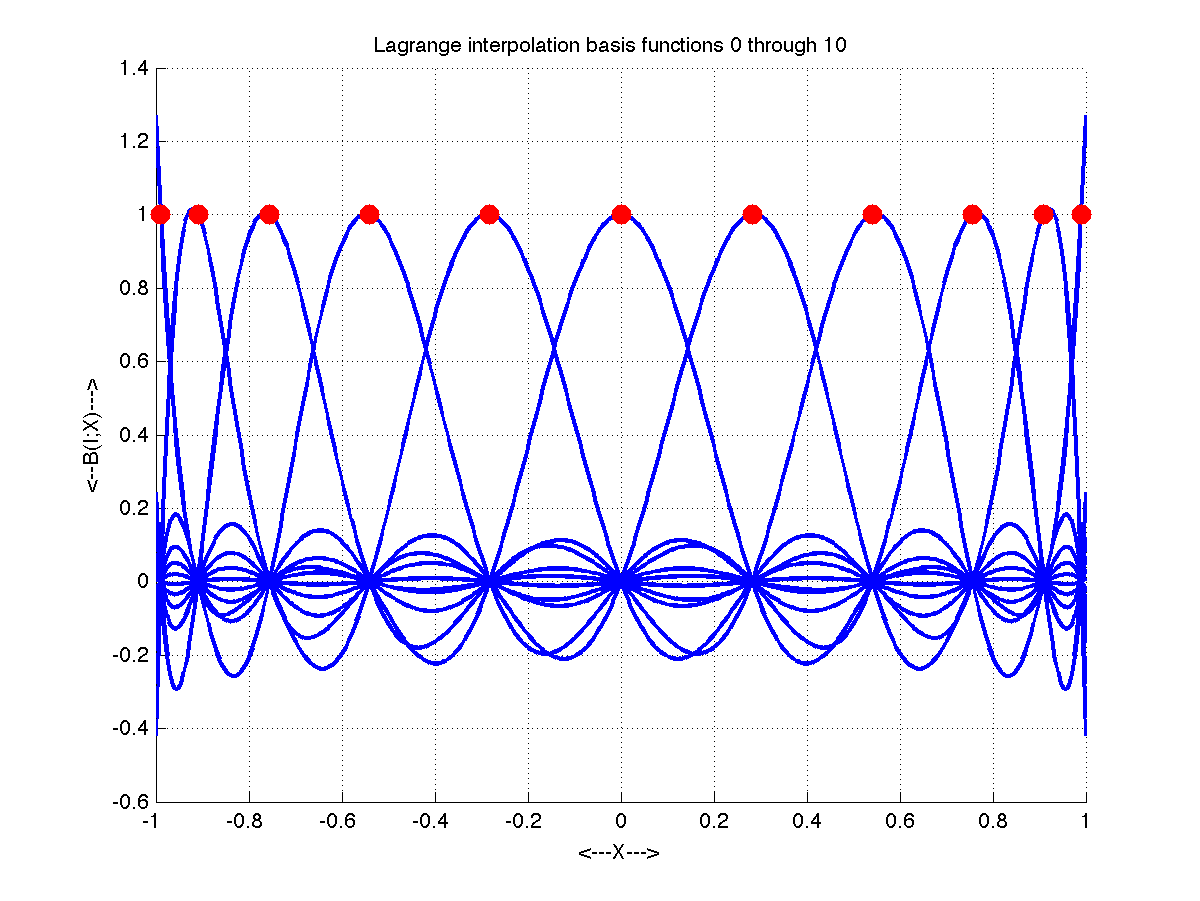
\includegraphics[width=8cm,height=6cm]{pics/lagrange_basis}\\
{\footnotesize A bázispolinomok ábrázolva.}
\end{center}
\paragraph{}
Felhasználva az előbb készített bázist, és a függvény értékeket, az interpolációs polinomot az alábbi formában kapjuk meg:$$L(x) = \sum_{i=0}^{n} f(x_i) \cdot l_i(x)$$
\begin{center}
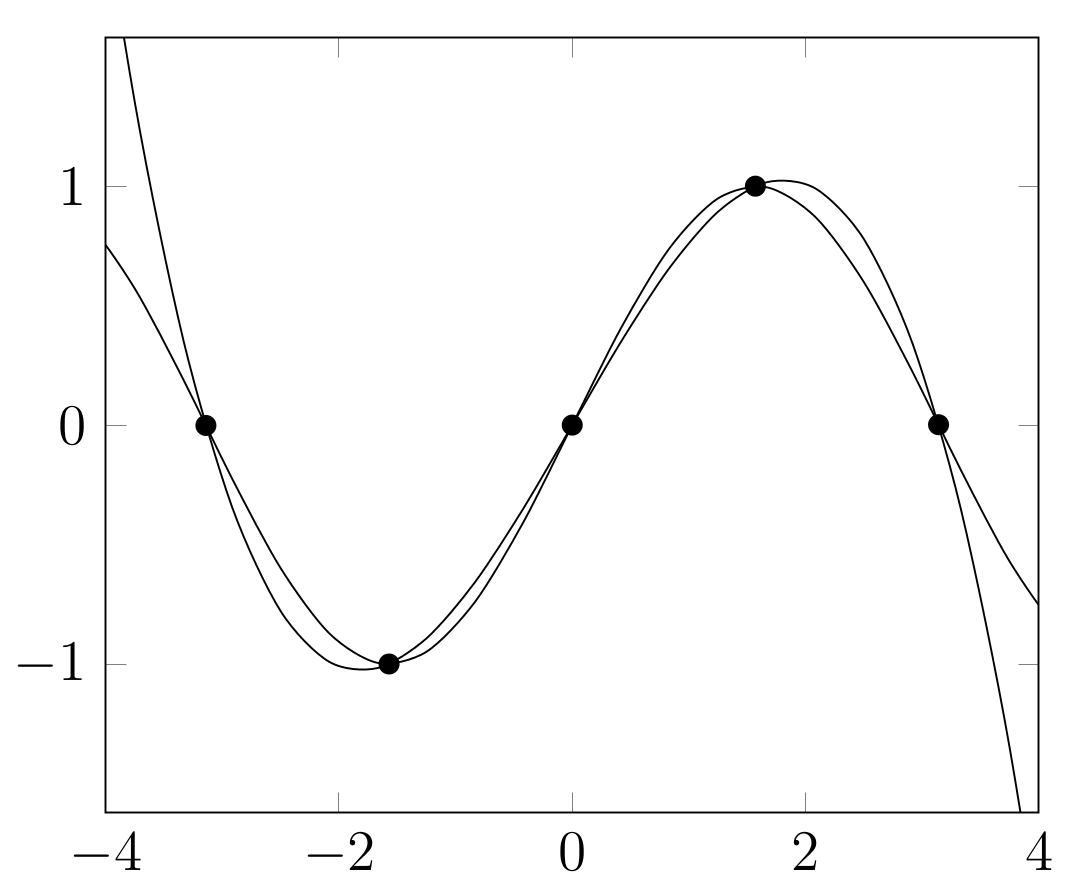
\includegraphics[width=8cm,height=6cm]{pics/polynomial_interpolation}\\
{\footnotesize Az interpolációs polinom és a függvény viszonya.}
\end{center}
\paragraph{}
A fenti bázist fel tudjuk használni, hogy kiterjesszük az interpolációt kétváltozós függvényekre, egyetlen kikötés, hogy az alappontok egy rácsot alkossanak. Ez azt jelenti, hogy az x tengelyre levetítve kapjuk az $x_0, \dots, x_n$ felosztást, ugyanígy az $y$ tengelyre $y_0, \dots, y_m$. Ekkor feltétel, hogy $\forall (x_i, y_j) \; i = 0 \dots n, \; j = 0 \dots m$ pontban tudjuk a függvény értékét. Innen az egy változónál használt elvet követve, készítünk $(n+1) \cdot (m+1)$ darab bázist, melyben fel tudjuk írni a közelítő függvényt.
\begin{center}
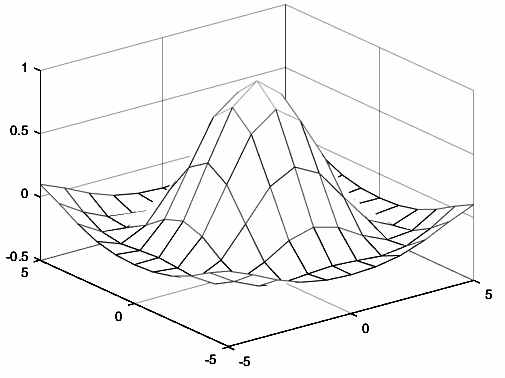
\includegraphics[width=10cm]{pics/bivariable_grid}\\
{\footnotesize Mintavételezés rácspontokban.}
\end{center}
\paragraph{}
Olyan bázist keresünk, melyekkel fel tudjuk írni az interpolációs polinomot az alábbi formában.
$$
L(x, y) = \sum_{i=0}^{n}\sum_{j=0}^{m}f(x_i, y_j) \cdot l_{i, j}(x, y)
$$
Az $l_{i, j}(x,y)$ bázis elkészítéséhez fel tudjuk használni a már egy változónál elkészített bázis polinomokat. Legyen
$$
p_i(x) = \prod_{k = 0, k \neq i}^{n}\frac{x-x_k}{x_i-x_k},\; q_j(y) = \prod_{k = 0, k \neq j}^{n}\frac{y-y_k}{y_j-y_k}
$$
A szorzatukból előáll a keresett bázis, hiszen az $l_{i, j}(x,y) = p_i(x)\cdot q_j(y)$ függvény az $(x_i, y_j)$ alappontban 1 értéket vesz fel, míg más alappontokban 0-át.

\subsection{Az interpolációs polinom Newton-alakja}
\paragraph{}
Ez a módszer is, a Lagrange-interpolációhoz hasonlóan, egy polinombázisban készíti el a közelítő függvényt. Előnye a gyors számítás, az osztott differenciák akár helyben is számolhatóak, új pont megadásakor nem kell teljesen újra számolni, elegendő csak az utolsó együtthatót kiszámolni. Hátránya, hogy nehezen terjeszthető ki több dimenzióra.
\paragraph{}
Először definiálnunk kell az osztott differenciát, $k$ darab pont osztott differenciájának a jelölése: $f[x_0, \dots, x_{k-1}]$. Legyenek $x_0, \dots, x_n$ alappontok, ekkor egy pontra az osztott differencia értéke önmaga, vagyis $[y_k] := y_k$. A $j$-ed rendű osztott differenciát az alábbi rekurzív képlet segítségével kapjuk meg:
$$
f[x_i, \dots, x_{i+j}] := \frac{f[x_{i+1}, \dots, x_{i+j}] - f[x_{i}, \dots, x_{i+j-1}]}{x_{j+i} - x_i}
$$
\begin{center}
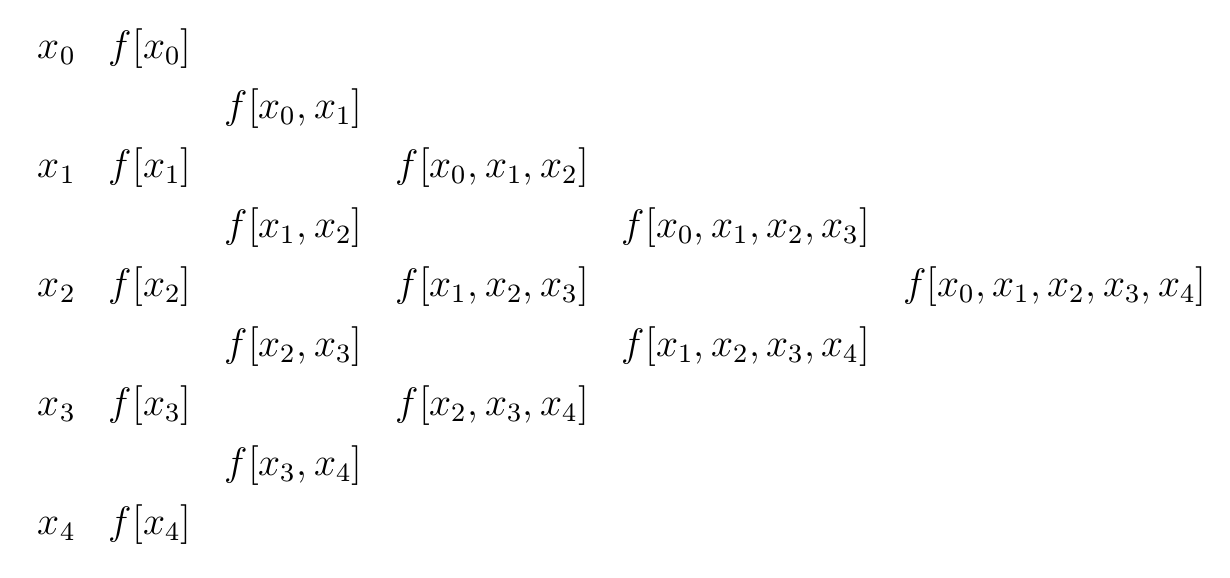
\includegraphics[width=10cm]{pics/divide_difference_table}\\
{\footnotesize Osztott differenciák táblázata.}
\end{center}
\paragraph{}
A bázis Lagrange módszerrel ellenkezően sokkal egyszerűbben felírható. Most a célunk egy könnyen bővíthető polinom bázis előállítása. Válasszuk az alábbi bázist.
$$
n_i = \prod_{j = 0}^{i}(x-x_j) \quad i \in [0, n - 1]
$$
Ekkor felhasználva az osztott differenciát felírhatjuk az interpolációs polinomot egyszerű formában.
$$
N(x) = f(x_0) + \sum_{k=1}^{n} f[x_0, \dots, x_k] \cdot n_i(x)
$$

\subsection{Alappontok választása}
\paragraph{}
A függvény és az azt közelítő polinom közötti eltérést szeretnénk a lehető legjobban lecsökkenteni, erre egy lehetőség az alappontok precíz megválasztása.
\paragraph{}
Vegyünk egy tetszőleges $f \in \mathbf{C}[a,b]^{n+1}$ függvényt, és közelítsük egy polinommal. Legyenek az alappontok $x_0, \dots, x_n$, ilyenkor egy tetszőleges belső pontban meg tudjuk becsülni a hibát.
$$
|f(x) - I_n(x)| \leq \frac{M_{n+1}}{(n+1)!} \cdot |\omega_n(x)|
$$
$$
M_{n+1} = \max\{|f^{n+1}(x)| \; : \; x \in [a,b]\} 
$$
$$
\omega_n(x) = (x-x_0)\cdot(x-x_1)\cdots(x-x_n)
$$
\begin{center}
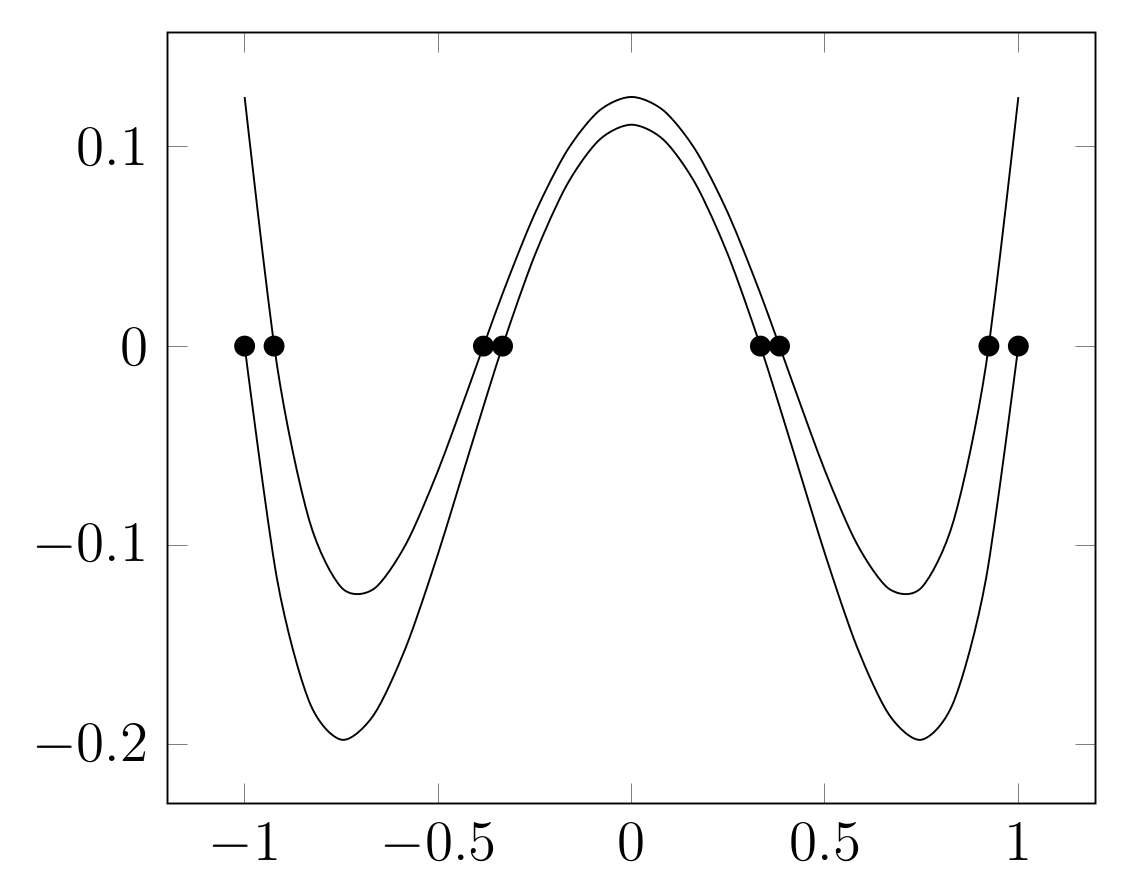
\includegraphics[width=8cm]{pics/chebyshev_and_even}\\
{\footnotesize $\omega$ függvények egyenletes és Csebisev alappontok esetén.}
\end{center}
\paragraph{}
A $T_n(x) = cos(n \cdot arccos(x)), \; x \in [-1, 1]$ függvényt Csebisev-polinomnak nevezzük. Rekurzióval meg tudjuk adni polinom formában is, $T_0(x)=1$, $T_1(x) = x$ és $T_n(x) = 2x \cdot T_{n-1}(x)-T_{n-2}(x)$.
\paragraph{}
$T_n$ főegyütthatója $2^{n-1} (n \geq 1)$, leosztva vele megkapjuk az 1 főegyütthatós Csebisev-polinomot $T^*_n(x) = \frac{1}{2^{n-1}} \cdot T_n(x)$.
Ezen $T^*_n(x)$ polinom tulajdonsága:
$$
\min\{ \|Q\|_\infty : \; Q \in P^{(1)}_n\} = \|T^*_n\|_\infty = \frac{1}{2^{n-1}}
$$
\paragraph{}
Ha a fenti hibaképletben az $\omega_n(x)$ helyére a $T^*_n(x)$ függvényt írjuk, akkor a hiba értéke kisebb lesz. Mivel $\omega_n(x)$ gyökei az alappontok, így a Csebisev-polinom gyökeit kell alappontnak választani. A gyököket a  trigonometrikus képlet segítségével tudjuk kiszámolni, az $n$-ed fokú polinom gyökei:
$$
x_k = cos(\frac{2 \cdot k + 1}{2 \cdot n} \cdot \pi) \quad k = 0, \dots , n-1
$$
\paragraph{}
Mivel a gyökök a $[-1, 1]$ intervallumon belül vannak, ezért lineáris transzformáció segítségével tudunk megfelelő alappontokat előállítani. Az $[a,b]$ intervallumra egy $f \in [-1,1] \rightarrow [a,b]$ függvény alkalmazásával tudjuk leképezni, mely $a$ és $b$ paraméter-ek segítségével az alábbi formában áll elő:
$$
f(x) = \frac{a+b}{2}+\frac{b-a}{2} \cdot x
$$
Elértük, hogy legyen $n$ darab alappontunk az $[a,b]$ intervallumon, melyekre el tudjuk így végezni az interpolációt. Ezekkel az alappontokkal készített polinom már sokkal jobb közelítést ad, a hibaképletbe behelyettesítve az ismert információkat kapjuk:
$$
|f(x)-I_n(x)| \leq \frac{M_{n+1}\cdot(b-a)^{n+1}}{(n+1)! \cdot 2^{2n+1}}
$$

\section{3D grafika}
\paragraph{}
A kezdeti számítógépek csak szöveges formában kommunikáltak a felhasználókkal, majd később született meg a grafikus ábrázolás, ami nagyban megkönnyítette a használatot. Ahogy fejlődtek a számítógépek, az egyre erősebb grafikus processzorok képesek már háromdimenziós ábrázolásra is. Ez nem tényleges háromdimenziós megjelenítést jelent, a legtöbb esetben egy három dimenziós jelenet egy adott pontból látható képét jeleníti meg.

\subsection{Modellek}
\paragraph{}
A pontábrázolás legelterjedtebb módszer a Descartes-féle koordináta-rendszer, melyben kitüntetett szerepe van az origónak, a rendszer középpontjának. Minden más egy háromelemű bázis lineáris kombinációjának segítségével adható meg. Az alapértelmezett jelölésben:
$$
O = \left( \begin{array}{c} 0\\ 0\\ 0 \end{array} \right)
$$
A három báziselem pedig:
$$
\mathbf{i} = \left( \begin{array}{c} 1\\ 0\\ 0 \end{array} \right) \quad \mathbf{j} = \left( \begin{array}{c} 0\\ 1\\ 0 \end{array} \right) \quad \mathbf{k} = \left( \begin{array}{c} 0\\ 0\\ 1 \end{array} \right)
$$
Ekkor a $P = (2, 1, 4)$ pontot a $\mathbf{p} = 2 \mathbf{i} + 1 \mathbf{j} + 4 \mathbf{k}$ vektor írja le.
\paragraph{}
A Polárkoordináta-rendszer esetében kitüntetett szerepe van az origónak, valamint két origó végpontú félegyenesnek. Ekkor a pontokat az alapponttól vett távolság, és a félegyenesekkel bezárt szög segítségével adjuk meg. Legismertebb alkalmazási területe a GPS rendszerek, ahol a Föld középpontja az alappont, a két félegyenessel bezárt szög pedig a földrajzi szélesség és a hosszúság.
\paragraph{}
Mivel mindkét rendszer a háromdimenziós teret írja le, így transzformációval páronként egymáshoz tudjuk rendelni őket.
Gömbkoordináta, vagyis háromdimenziós polárkoordináta rendszerből Descartes-féle koordináta-rendszerbe az alábbi $(\mathbb{R} \times \mathbb{R} \times \mathbb{R}) \rightarrow (\mathbb{R} \times \mathbb{R} \times \mathbb{R})$ függvény segítségével tudjuk transzformálni a pontjainkat.
$$
\left( \begin{array}{c}
	R \\
	\theta \\
	\phi \end{array}
\right)
\rightarrow
\left( \begin{array}{c}
	R \cdot \sin \theta \cdot \cos \phi \\
	R \cdot \sin \theta \cdot \sin \phi \\
	R \cdot \cos \theta
\end{array} \right)
$$
Természetesen a másik irányba is létezik egy $(\mathbb{R} \times \mathbb{R} \times \mathbb{R}) \rightarrow (\mathbb{R} \times \mathbb{R} \times \mathbb{R})$, így a Gömbkoordináta rendszerbeli pontjainknak tudunk egy Descartes-féle koordináta-rendszerbeli pontot megfeleltetni.
$$
\left( \begin{array}{c}
	x \\
	y \\
	z \end{array}
\right)
\rightarrow
\left( \begin{array}{c}
	\sqrt{x^2+y^2+z^2} \\
	\arccos{\frac{z}{\sqrt{x^2+y^2+z^2}}} \\
	\arccos{\frac{x}{\sqrt{x^2+y^2}}}
\end{array} \right)
$$
A továbbiakban csak a Descartes-féle koordináta-rendszert használjuk, mert a használt alkalmazásprogramozási interfész, röviden API, szintén ezt használja.
\paragraph{}
Programozásnál sokszor használunk közelítést, ez történik a modellezés esetén is. Az alakzatokat poligonok segítségével közelítjük, melyeket könnyen tudunk tárolni a pontok és köztük futó élek segítségével. Azonban ezeket az alakzatokat el is kell helyeznünk a térben, ehhez pedig szükségünk van arra, hogy eltoljuk, átméretezzük és elforgassuk őket. Ezeket a transzformációkat egy mátrixszorzásnak feleltetjük meg, így sok pontra is gyorsan el tudjuk őket végezni.
\paragraph{}
Nézzük az alap transzformációkat. Az eltolás lényege, hogy egy $P = (x_1, y_1, z_1)$ pontot egy adott $\mathbf{d} = (d_x, d_y, d_z)$ vektorral eltoljuk, és kapjuk a $P' = (x_2, y_2, z_2) = P + \mathbf{d}$ pontot. Ezt a transzformációt egy $\mathbb{R}^{4\times4}$ mátrix segítségével tudjuk végrehajtani, azonban a művelet végrehajtása előtt, ahhoz hogy a szorzás értelmezve legyen, a $P$ pontot egy negyedik elemmel, egy egyessel is ki kell egészíteni. Így áll elő az alábbi képlet.
$$
\left( \begin{array}{cccc}
	1 & 0 & 0 & d_x \\
	0 & 1 & 0 & d_y \\
	0 & 0 & 1 & d_z \\
	0 & 0 & 0 & 1 \\
\end{array} \right)
\cdot
\left( \begin{array}{c}
	x_1 \\
	y_1 \\
	z_1 \\
	1 \end{array}
\right)
=
\left( \begin{array}{c}
	x_1 + d_x \\
	y_1 + d_y \\
	z_1 + d_z \\
	1 \end{array}
\right)
$$
\paragraph{}
Forgatáskor egy adott tengely körül egy szöggel forgatjuk el a pontokat. Elegendő csak a tengelyek körüli forgatást levezetni, ugyanis velük bármilyen másikat le tudunk írni. Első lépésként el kell tolnunk a forgástengelyt az origóba, majd két főtengely körüli forgatással a forgástengelyt a harmadik vonalába transzformáljuk, majd elvégezzük a forgatást. Aztán az első két forgatás, és az eltolás inverzét alkalmazva megkapjuk a kívánt eredményt. A főtengelyek körüli forgatások rendre a következőek:
$$
\left( \begin{array}{cccc}
	\cos\alpha & -\sin\alpha & 0 & 0 \\
	\sin\alpha & \cos\alpha & 0 & 0 \\
	0 & 0 & 1 & 0 \\
	0 & 0 & 0 & 1 \\
\end{array} \right)
\quad
\left( \begin{array}{cccc}
	\cos\alpha & 0 & \sin\alpha & 0 \\
	0 & 1 & 0 & 0 \\
	-\sin\alpha & 0 & \cos\alpha & 0 \\
	0 & 0 & 0 & 1 \\
\end{array} \right)
\quad
\left( \begin{array}{cccc}
	1 & 0 & 0 & 0 \\
	0 & \cos\alpha & -\sin\alpha & 0 \\
	0 & \sin\alpha & \cos\alpha & 0 \\
	0 & 0 & 0 & 1 \\
\end{array} \right)
$$
\paragraph{}
Szükségünk van még arra, hogy egy alakzat méretét meg tudjuk változtatni, akár azonos, akár tengelyenként különböző mértékkel. Ismét elegendő, hogy az origóban lévő alakzatot méretezzük át, hiszen eltolással oda és vissza tudjuk helyezni.  Az eddigiekhez hasonlóan, ezt is feltudjuk írni egy $4 \times 4$-es mátrix formájában.
$$
\left( \begin{array}{cccc}
	s_x & 0 & 0 & 0 \\
	0 & s_y & 0 & 0 \\
	0 & 0 & s_z & 0 \\
	0 & 0 & 0 & 1 \\
\end{array} \right)
$$
\paragraph{}
Mivel minden transzformáció mátrixa azonos méretű, így könnyen végre tudjuk hajtani őket egymás után, akár komplex transzformációt is létre tudunk hozni, a megfelelő mátrixok összeszorzásával. Amikor több transzformációt hajtunk végre egymás után, akkor azok mindig jobbról balra fognak sorban következni a végrehajtásban. Például ha szeretnénk a $P$ alakzatod a felére csökkenteni, az $X$ tengely körül elforgatni $90^{\circ}$-al, majd eltolni a $(1,5,-2)$ pontba, akkor azt a következő módon tehetjük meg:
$$
\left( \begin{array}{cccc}
	1 & 0 & 0 & 1 \\
	0 & 1 & 0 & 5 \\
	0 & 0 & 1 & -2 \\
	0 & 0 & 0 & 1 \\
\end{array} \right)
\cdot
\left( \begin{array}{cccc}
	\cos(\frac{\pi}{2}) & -\sin(\frac{\pi}{2}) & 0 & 0 \\
	\sin(\frac{\pi}{2}) & \cos(\frac{\pi}{2}) & 0 & 0 \\
	0 & 0 & 1 & 0 \\
	0 & 0 & 0 & 1 \\
\end{array} \right)
\cdot
\left( \begin{array}{cccc}
	0.5 & 0 & 0 & 0 \\
	0 & 0.5 & 0 & 0 \\
	0 & 0 & 0.5 & 0 \\
	0 & 0 & 0 & 1 \\
\end{array} \right)
\cdot
P
$$

\subsection{Megjelenítés}
\paragraph{}
Alakzatokból a fentebb ismertetett transzformációk segítségével létre tudjuk hozni a háromdimenziós képet, azonban ezt még nem lehet megjeleníteni, hiszen a legtöbb számítógép kimeneti perifériája egy monitor, ami csak kétdimenziós képmegjelenítést támogat. Így csak egy térbeli hatást tudunk kelteni, például azzal, hogy a közelebbi tárgy eltakarja a távolabbit, ami messzebb van, az kisebbnek látszódik.
\paragraph{}
A továbbiakban egy összetett struktúrát, a vertexeket fogjuk használni, mely tartalmazza a pont koordinátáját, a színét és a normálisokat. Az első komponens, koordináta, adja meg, hogy a térben hol helyezkedik el az adott pont. A második komponens a pont színe, vagy textúrázott objektum esetén a koordinátái. A normálisok egy felületre - a pontok esetében arra a felületre melynek részei - merőleges vektorok. Segítségükkel tudunk fényeket, visszaverődést meghatározni.
\paragraph{}
A grafikus szerelőszalag feladata, hogy a vertexekből előállítson egy kétdimenziós képet. Mivel ez egy összetett feladat, ezért több részfeladatra bontás és csővezeték használatával párhuzamosítható és gyorsítható.
\begin{center}

\includegraphics[width=6cm]{pics/vertex_transformation}\\
{\footnotesize A vertexek transzformációja}
\end{center}
\paragraph{}
Legelső lépés a vertexek sorba állítása a feldolgozáshoz, ezután egymás után haladnak sorban a csővezetékben. Innentől vertexenként külön-külön végrehajtódnak a különböző műveletek. A vertex-feldolgozó egység bemenete egy vertex (pozíció, szín, normális, egyebek), kimenete egy már megfelelően transzformált vertex. Megjelenítéshez szükség van három fő transzformációra, melyek mátrixszorzásként hajtódnak végre a vertex pozícióján. Az világban megfelelő helyre történő transzformálás az első, az előző részben bemutatott egyszerű transzformációk szorzataként áll általában elő. Ezután a nézet transzformáció következik, ami azt állítja be, hogy mi melyik pontból, és hogyan lássuk az elkészített jelenetet. Utolsó lépésként pedig az előállított végső jelenetet vetíti le a kétdimenziós vásznunkra. A három transzformációt elvégezve az egység továbbküldi a vertexet.
\begin{center}
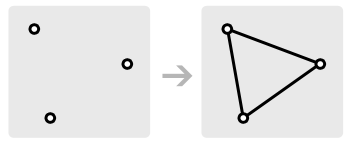
\includegraphics[width=6cm]{pics/shape_assembly}\\
{\footnotesize Alakzatok felépítése}
\end{center}
\paragraph{}
Már elkészített transzformált vertexekből háromszögeket épít fel a következő egység, azért háromszöget, mert azok biztosan egy síkon vannak, így könnyű velük dolgozni. Az elkészült háromszögekből ezután levágja azokat a részeket, melyek kilógnak a látótérből. Ügyelve arra, hogy továbbra is háromszögek maradjanak, ezért, ha levágás után négyszög keletkezne, akkor azt két háromszögre bontja fel. Az előállított síkidomok ezután további feldolgozásra haladnak tovább a szalagon.
\begin{center}
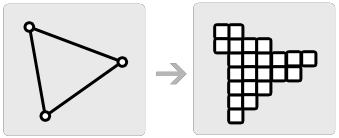
\includegraphics[width=6cm]{pics/rasterization}\\
{\footnotesize Raszterizáció}
\end{center}
\paragraph{}
Raszterizáció lényege, hogy az elkészült háromszögeket a lehető legkisebb egységekre bontsa. Első lépésben meghatározza egy háromszögről, hogy mely pixelek tartoznak hozzá, vagyis vannak benne. Ezután a háromszög három csúcspontjának színe és távolsága alapján meghatározza minden fragment színét, majd innen az adatokat egy bufferba küldi tovább. A kép frissítésekor a buffer tartalma alapján ki tudjuk rajzolni a képernyőre a kívánt alakzatot.

\section{Formális nyelvek és fordítóprogramok}
\paragraph{}
A matematika világában mindent megpróbálunk formálisan leírni, mert csak így tudjuk a fogalmakat használni és bizonyítani a tételeket. A formális nyelvekkel is ugyanígy járunk el, megpróbálunk szabályokat felírni, mely segítségével a nyelv levezethető. Ezzel el tudjuk dönteni, hogy egy adott, formális nyelvben vett szó, egy adott nyelvhez tartozik-e. Ez a folyamat történik akkor is, mikor a fordító program az általunk írt kódot elemzi és készíti el a futtatható állományt. Ekkor a programunk lesz a szó, és a fordítóprogram különböző elemzői döntik el, hogy valóban az adott programnyelvbe tartozik-e a kódunk.

\subsection{Nyelvek leírása formálisan}
\paragraph{}
A nyelvek alapjai a szimbólumok, a nem üres véges halmazuk pedig az ábécé. Egy $L$ ábécé feletti szavak halmazát $L^+$-al jelöljük, ha az üres szót is belevesszük, akkor $L^*$-al jelöljük.
\paragraph{}
Formális nyelveket le tudunk írni nyelvtanokkal, mely megadja a nyelv ábécéjét, terminális szimbólumok, és azokat a szabályokat, melyek segítségével az adott kezdő szimbólumból el tudunk jutni a nyelv által generált összes szóig. Továbbiakban $G$ nyelvtan egy olyan négyes $(N, T, P, S)$, ahol $T$ és $N$ a terminális és nemterminális szimbólumok ábécéi, feltétel, hogy diszjunktak. $P$ a szabályok halmaza, $(N \cup T)^+ \rightarrow (N \cup T)^*$ függvények, $S \in N$ pedig a kezdőszimbólum.
\paragraph{}
Az $(X \rightarrow Y)$ szabály jelentése, hogy ha $X$-et le tudjuk vezetni, akkor $Y$-t is, ezt rekurzívan követve, ha egy szóról azt kapjuk, hogy $S$-ből levezethető, akkor a nyelv egyik szava. Könnyebb olvashatóság céljából, ha több olyan szabály létezik, mely bal oldala azonos, akkor őket össze tudjuk vonni, és a jobb oldalakat $|$-el elválasztva soroljuk fel.
\paragraph{}
Az alábbi példán az egész számokon értelmezett alapműveletek nyelvét mutatjuk be. Legyen $G=(N, T, P, S)$, ahol
$$
\begin{array}{rl}
T= & \{0, 1, 2, 3, 4, 5, 6, 7, 8, 9, +, -\} \\
N= & \{Start, Number, Digit, Operator\} \\
S= & Start \\
P= & \{Start \rightarrow Number | Number \; Operator \; Start, \\
&\; Number \rightarrow Digit | Digit \; Number, \\
&\; Digit \rightarrow 0 | 1 | 2 | 3 | 4 | 5 | 6 | 7 | 8 | 9, \\
&\; Operator \rightarrow + | -|\cdot\}
\end{array}
$$
\paragraph{}
A szabályok alkalmazásával minden szóhoz elő tudunk állítani egy szintaxisfát, melynek a gyökerében a kezdőszimbólum, a leveleiben pedig nemterminális szimbólumok állnak. Ez a fa nem minden esetben egyértelmű, léteznek olyan szavak, melyekhez több fa is tartozik. Példákban a $2+3\cdot4$ szóhoz két különböző fát tudunk előállítani, melyek később fontos szerepet töltenek be az elemzés során. Ilyenkor szükséges, hogy további elemzéshez a megfelelő fát küldjük tovább, a helyes eredmény érdekében.
\begin{center}
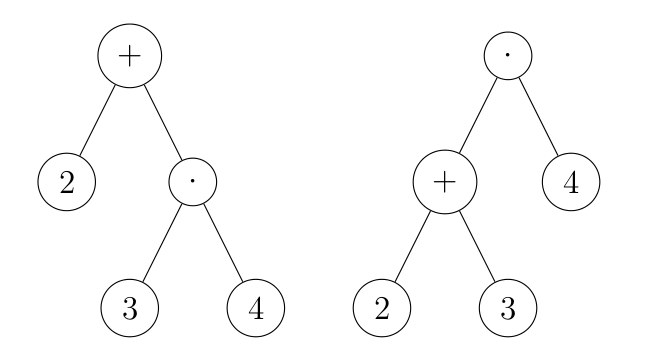
\includegraphics[width=8cm]{pics/syntax_tree}\\
{\footnotesize A $2+3\cdot4$ kifejezés két szintaxisfája.}
\end{center}

\subsection{Fordítás menete}
\paragraph{}
A fordítás első lépése a lexikális elemzés, melynek feladata, hogy a bemenetről eldöntse, megfelel a nyelv ábécéjének, és szimbólumokra, úgynevezett tokenere bontsa azt. Ennek segítségére reguláris kifejezéseket használunk, melyekkel könnyen fel tudunk írni akár bonyolultabb szimbólumokat is.
\paragraph{}
Például a $(\backslash +|-)?[0-9]+(\backslash.[0-9]+)?$ kifejezés írja le a számokat. Három rész különböztethető meg, előjel, egészrész és törtrész. Az előjelet $(\backslash+|-)?$ írja le, ahol a $+$ és $-$ az előjeleknek felel meg, a $\backslash$ az úgynevezett escape karakter, a $+$ jelnek kitüntetett jelentése van, $|$ jelöli, hogy a kettő közül az egyik, ha többet írunk egymás utána, akkor a sok közül az egyiket jelenti. Sok elem esetén listát használhatunk, $[a-z]$, ez hasonló az előzőhöz, a sok elem közül az egyikre illeszkedik. A kifejezés végén álló $?$ az előtte álló részről megengedi, hogy nullaszor vagy egyszer szerepeljen. Hozzá hasonlóan a $+$ és $*$ jelek is a mennyiséget módosítják, míg a $+$ kifejezés egyszer vagy többször, addig a $*$ megengedi, hogy egyszer sem szerepeljen. A kifejezés $[0-9]+$ része a pozitív egész számokat írja le, az utolsó része pedig, hogy a pont után másik egész szám áll.
\paragraph{}
Miután a bemenetet tokenekre bontottuk, meg kell őket feleltetnünk a $P$ halmazban szereplő szabályoknak. A szabályok alkalmazása mentén előállítjuk a szintaxis fát, amennyiben az adott bemenet a nyelv egy szava.
\paragraph{}
Szemantikus elemzést azért végzünk, hogy az elkészített grammatika egyszerűbb legyen, és egyéb olyan feladatokat teljesítsen, melyeket szükséges elvégezni, de a szintaktikus elemzéskor nem volt rá lehetőségünk. Ez tipikusan kifejezések típusának helyességének ellenőrzése, újra deklarálás, vagy a nem deklarált változók felismerése. Ezek egyszerű ellenőrzésének érdekében bevezetjük a szimbólumtáblát, mely feladata, hogy számon tartsa, mely függvények, változók vannak jelenleg definiálva, és mi az ő típusuk.
\paragraph{}
A lexikális, szintaktikus és szemantikus elemzés után már biztosítva van, hogy a fordítás lehetséges, ilyenkor az adott nyelvünket bizonyos szabályok alapján egy másik nyelvre tudjuk fordítani, mely lehet akár már futtatható kód, vagy még csak egy köztes nyelv, amiből egy másik fordítóprogram segítségével futtatható kódot kapunk.

\subsection{Matematikai függvények formális nyelve}
\paragraph{}
A függvények interpolációjához szükségünk van arra, hogy a programban a matematikai függvényeket feltudjuk ismerni, kitudjuk értékelni. Erre az előbb bemutatott formális nyelv modellt használjuk fel. Jelölje a $G=(N, T, P, S)$ a matematikai függvények nyelvét, már csak az egyes részeket kell definiálnunk.
\paragraph{}
Az ábécénk most tokenekből fog állni, melyekre illeszkedő reguláris kifejezéseket adunk meg.
$$
T=\{var, num, open, close, add, min, mul, div, pow, abs, sin, cos, tg, ctg\}
$$
Meg kell adnunk minden elemnek a reguláris kifejezését, azért, hogy a lexikális elemző fel tudja ismerni.
$$
\begin{array}{rlrl}
var & ::= x|y & num & ::= [0-9]+(\backslash.[0-9]+)? \\
open & ::= \backslash( & close & ::= \backslash)\\
add & ::= \backslash+ & min & ::= -\\
mul & ::= \backslash* & div & ::= \backslash\backslash\\
pow & ::= \backslash\wedge & abs & ::= abs\\
sin & ::= sin\ & cos & ::= cos\\
tg & ::= tg & ctg & ::= ctg
\end{array}
$$
Következő lépés, a szabályokban használt nemterminális szimbólumok megadása, ügyelve arra, hogy ezen halmaz metszete a terminális szimbólumok halmazával üres legyen.
$$N=\{Start, Binary, Unary, Expression\}$$
A nemterminális és terminális szimbólumok ismeretében meg tudjuk konstruálni a nyelv szabályait. Az $S=Start$ választásával, az alábbi formát ölti a nyelvtan:
$$
\begin{array}{rl}
P= & \{Start \rightarrow Expression, \\
&\; Expression \rightarrow open \; Expression \; close, \\
&\; Expression \rightarrow Binary, \\
&\; Expression \rightarrow Unary, \\
&\; Expression \rightarrow var, \\
&\; Expression \rightarrow num, \\
&\; Binary \rightarrow Expression \; add \; Expression, \\
&\; Binary \rightarrow Expression \; min \; Expression, \\
&\; Binary \rightarrow Expression \; mul \; Expression, \\
&\; Binary \rightarrow Expression \; div \; Expression, \\
&\; Binary \rightarrow Expression \; pow \; Expression, \\
&\; Unary \rightarrow min \; Expression, \\
&\; Unary \rightarrow abs \; Expression, \\
&\; Unary \rightarrow sin \; Expression, \\
&\; Unary \rightarrow cos \; Expression, \\
&\; Unary \rightarrow tg \; Expression, \\
&\; Unary \rightarrow ctg \; Expression\}
\end{array}
$$
A $var$ és $num$ tokeneket úgynevezett szemantikus értékkel is ellátjuk, itt tároljuk, hogy melyik változóról van szó, $x$ vagy $y$, illetve, hogy az adott számnak mi az értéke. A nyelvhez előre elkészített szimbólumtábla tartozik, melyben az egyes műveletek és függvények kiszámításának módja található. Megtalálható még benne az egyes bináris műveletek precedenciája, mely segít a helyes szintaxisfa előállításában.

\subsection{Precedencia elemző}
\paragraph{}
A precedenciák ismeretében fel kell építenünk a helyes szintaxisfát, lásd $2+3\cdot4$ esete, csak az egyik változata eredményezte a helyes végeredményt. Ilyen feladatnak többféle megoldása is létezik, futási idő, fa felépítések iránya és előre olvasott szimbólumok száma alapján. A programban egy LR(1) parser, a precedencia elemőzre esett a választás. Az L jelentése, hogy a bemenetet balról jobbra olvasva, visszalépés nélkül elemzi, az R jelentése, hogy jobboldali levezetést használ, vagyis a fát lentről felfelé építi fel. Az 1-es jelentése, hogy egyetlen szimbólum előreolvasása után dönti el, hogy a bemenetet kell léptetnie, vagy a jelenlegit redukálnia.
\paragraph{}
Az elemző két rekurzív függvény segítségével lett megvalósítva, az első feladata az elemi kifejezések felismerése, ezek jelen esetben lehetnek előjeles számok, változók, függvények, valamint zárolójelek közötti összetett kifejezések. Ezek felismerésére szolgál a másik rekurzív függvény, mely egy adott precedenciánál nagyobb összetartozó részeket ismeri fel. Az algoritmus implementációja Fejlesztői fejezetben további információ található.
\paragraph{}
Utolsó lépés az előállított fa segítségével kiértékelni a függvényt adott pontban. A mélységi bejárás algoritmusának postorder változatával könnyen el is tudjuk ezt végezni, hiszen szülő mindig egy részkifejezés főművelete, így azt az után kell elvégezni, hogy a gyerekeiben lévő műveletet elvégeztük. Egészen addig kell rekurzívan lefelé mennünk, amíg el nem érünk egy levélhez, ahol két lehetőség van. Az első, hogy a levélben egy változó van, ekkor a szemantikus érték alapján kiválasztjuk, hogy melyik változó értékét kell behelyettesíteni, a másik lehetőség, hogy egy szám áll ott, ilyenkor csak a szemantikus értékkel számolunk tovább.

\chapter{Felhasználói dokumentáció}

\section{Bemutatás}

\section{Telepítés}

\subsection{Rendszer követelmények}
\paragraph{}
Az alkalmazás működéséhez és megjelenítéshez az futtató számítógépnek az alábbi követelményeket teljesíteni-e kell: \\ \\
\begin{tabular}{l | l}
Operációs rendszer & Windows 7, 8, 10 vagy Linux \\
Felbontás & Legalább 1280x1024, ajánlott 1980x1080 \\
Processzor & Az optimális működéshez 2 szálat támogató, 3GHz órajelű \\
Grafikus kártya & OpenGL 4.0-et támogató, legalább 512MB memóriával rendelkező \\
Háttértároló & Nem igényel a futtatható állomány méreténél nagyobb területet \\
Internet & Nincs szükség internetkapcsolatra \\
Bemenet & Billentyűzet és egér szükséges
\end{tabular}
Amennyiben valamelyik feltétel nem teljesül, úgy a program kényelmes működése nem garantált.

\subsection{Egyéb függőségek}
\paragraph{}
A program nem igényel telepítést, elegendő az operációs rendszerhez tartozó futtatható állományt a számítógépre másolni. Mivel a Qt keretrendszer segítségével készült a program, ezért egyéb segédfájlok meglétét igényli.
\paragraph{}
Ezek a fájlok is megtalálhatóak a futtatható állomány mellett, csak a program által elérhető mappába kell őket másolni. Ez operációs rendszerenként eltérő, van ahol elegendő a futtatható állomány mellé helyezni, viszont egyes esetekben elkerülhetetlen, hogy rendszermappába helyezze őket.
\paragraph{}
Amennyiben nem sikerül a másolással megoldani a függőségeket, úgy a Qt keretrendszer oldaláról letölthető a Qt 5.6-os verziója, mely letöltése és telepítése elhelyezi a szükséges segédfájlokat a megfelelő mappákban.

\section{Használat}

\subsection{Funkciók leírása}
\paragraph{}
A programot az Interpolator futtatható állomány segítségével indíthatja el, ekkor megjelenik a főablak.
Itt a bemeneti információkat különböző módon adhatja meg. A módok közötti az elhelyezett fülek segítségével tud váltani.
\paragraph{}
Ajánlott először az alappontokat megadni. A kényelmesebb megoldás, ha a Felosztás opciót választja. Ekkor az intervallumok két végpontját és az alappontok számának megadása után térjen az értékek megadása részhez.
\begin{center}
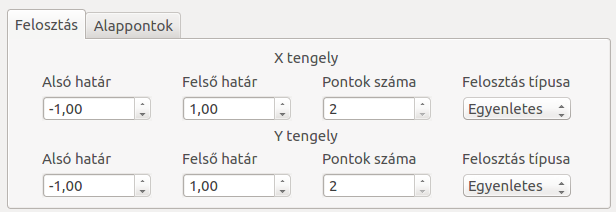
\includegraphics[width=7cm]{pics/gui/partition1}  \\
{\footnotesize Felosztás fül} 
\end{center}
\paragraph{}
Amennyiben szeretné manuálisan beállítani az alappontokat, úgy a másik fül segítségével, először az alappontok számának megadása után tudja megadni a pontok helyzetét. Ügyeljen arra, hogy ne maradjon üresen mező, valamint ne legyenek azonos alappontok sem.
\begin{center}
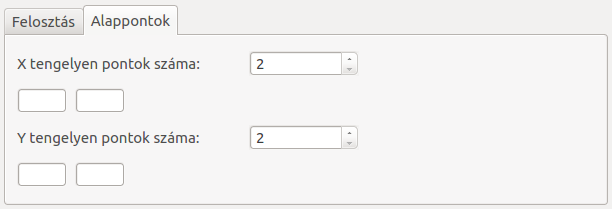
\includegraphics[width=7cm]{pics/gui/partition2}  \\
{\footnotesize Alappontok fül} 
\end{center}
\paragraph{}
Miután megadta az alappontokat, az értékek megadására is két módszert nyújt a program. Amennyiben ismert a függvény, úgy elegendő azt a Függvény fül alatt található szövegdobozba beírni, majd a Kirajzolás gomb lenyomására megjelenik.
\paragraph{}
Ismeretlen függvény esetén az Értékek fül alatt tudja megadni az alappontokban felvett értékeket. Amennyiben minden mezőt kitöltött, a Kirajzolás gomb segítségével megjelenítheti az interpoláció eredményét.
\paragraph{}
A menüben található Mentés és Betöltés gombok használatával van lehetősége a jelenlegi konfiguráció lementésére, valamint ismételt betöltésére. A gomb lenyomása után egy párbeszédablak segítségével választhatja ki a kívánt fájlt.
\paragraph{}
A program egyváltozós függvény megjelenítését is támogatja, ezt az Egyváltozós gomb lenyomásával érhetjük el. Ekkor a felületen a második változóra vonatkozó mezők kikapcsolnak, és csak az egyik változóra vonatkozó adatokat kell megadnia.
\paragraph{}
Szemléltetés céljából, a Lépések mutatása gombbal tud be- és kikapcsolni egy segédfunkciót. A bekapcsolásakor a megjelenítés folyamata párbeszédablakokban érdekes és hasznos információkat jelenít meg.
\begin{center}
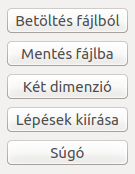
\includegraphics[width=5cm]{pics/gui/menu}  \\
{\footnotesize A menü} 
\end{center}
\paragraph{}
A programot a főnézet bezárógombjának segítségével tudja megállítani. Ekkor az összes többi ablak is bezáródik, valamint a program terminál.
\subsection{Hibaüzenetek jelentése}

\chapter{Fejlesztői dokumentáció}

\section{Feladat specifikációja}
\paragraph{}
A feladat egy olyan grafikus alkalmazás elkészítése, mely a felhasználó által megadott adatokból elkészíti, és megjeleníti az interpolációs közelítést, valamint ha lehetséges, azt a függvényt is, melyet közelít.

\subsection{Követelmények}
\paragraph{}
Kényelmi funkciók miatt a felhasználónak több lehetőséget kell biztosítani az információk megadására. Az alappontokat megadhatja manuálisan is, de legyen lehetősége az intervallum és a pontok számával is, ekkor automatikusan állítódjanak be a pontok.
\paragraph{}
Mivel a függvény közelítése a cél, ezért annak megadására legyen lehetőség, ilyenkor a függvény alappontban felvett értékeivel lehet tovább számolni. Ismeretlen függvények miatt biztosítson lehetőséget a tényleges értékek bevitelére.
\paragraph{}
Alapértelmezetten egy háromdimenziós térben, egy felület formájában jelenjenek meg a függvények. Nem mindig van szükség erre, egyváltozós függvények esetén elegendő egy kétdimenziós koordináta rendszerben ábrázolni egy folytonos vonal formájában.
\paragraph{}
Az újrahasználás, és hordozhatóság céljából tudjuk menteni az adatokat fájlokba, melyekből később bármikor újra be tudjuk állítani az adatokat. Nem szükséges az információkat lekódolni, mert nem tartalmaznak érzékeny információt.
\paragraph{}
Egyszerű személyre szabás és használhatóság érdekében külön ablakokban jelenítse meg az információkat, a felhasználó az ablakokat mozgathatja és átméretezheti.
\paragraph{}
A programnak több platformon is működnie kell, ezzel növelve a lehetséges felhasználók számát. Feltételezhetjük, hogy a futtató számítógép rendelkezik grafikus megjelenítővel és támogatja az OpenGL szabványt.

\subsection{Felhasználói esetek}
\paragraph{}
A programot egyidejűleg egyetlen felhasználó használja, aki minden funkciót elér. A következő ábrán látható a rendszer összes felhasználói esetét tartalmazó UML diagram. Alatta a funkciók részletes leírása következik.
\begin{center}
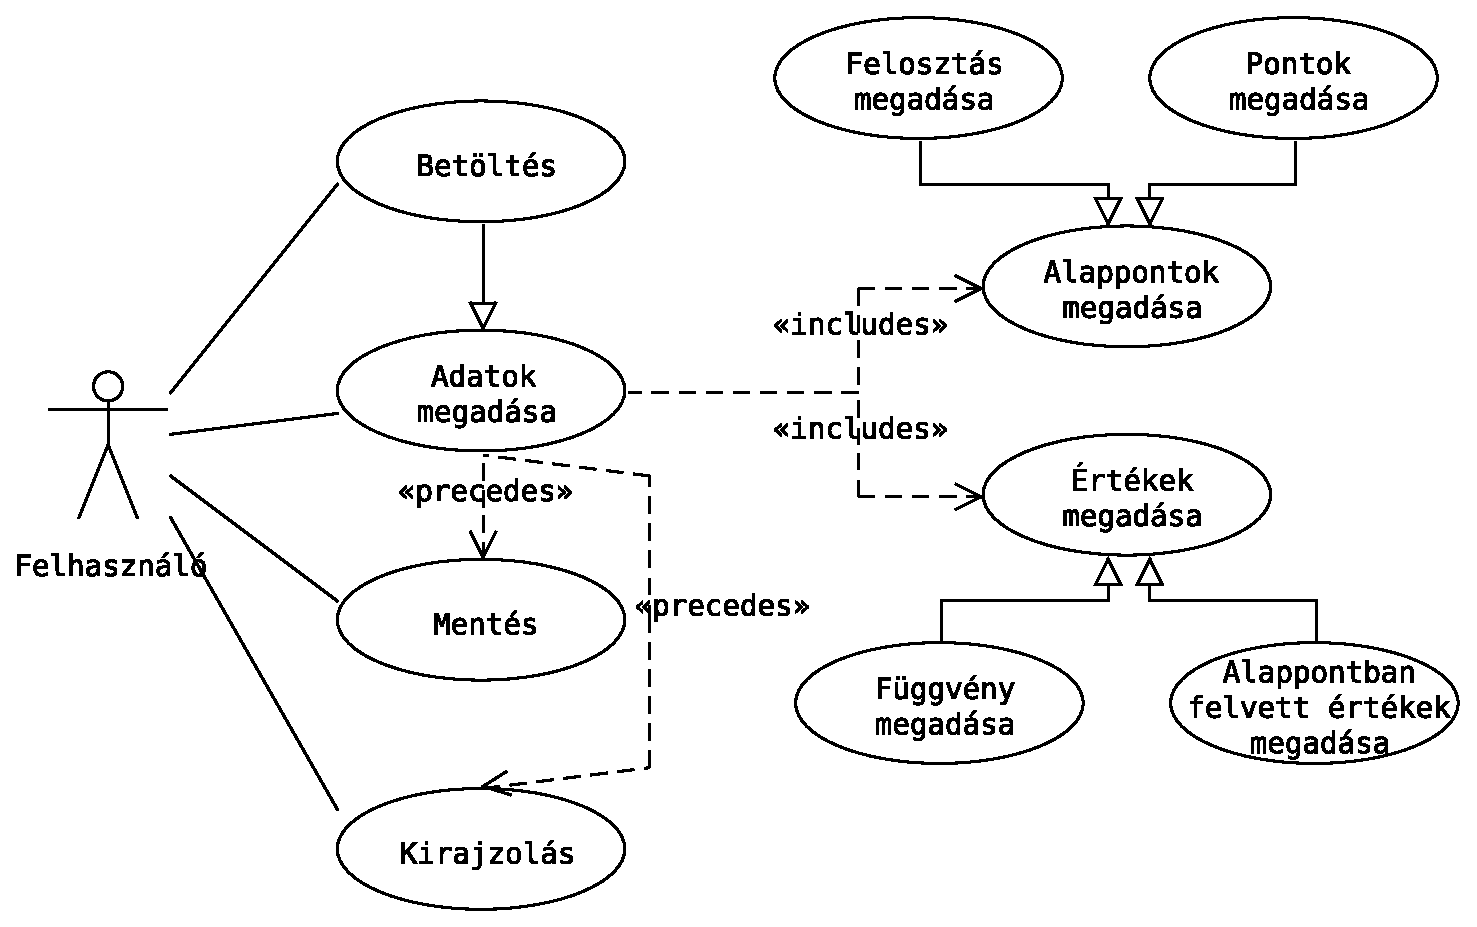
\includegraphics[width=11cm]{pics/uml/use_case}\\
{\footnotesize A felhasználói esetek}
\end{center}

\subsubsection{Adatok megadása funkció}
\paragraph{}
Nincs előfeltétele, így bármikor végrehajtható. Két fő részből áll, az interpolációhoz szükséges adatokat kell megadnia a felhasználónak. Ezek az alappontok és ezen pontokban felvett függvényérték. Ha bármely szükséges információ hiányzik, a program hibajelzéssel közli.

\subsubsection{Alappontok megadása funkció}
\paragraph{}
Az interpolációhoz szükséges mintavételezési pontok megadása. A felhasználói kényelem céljából megadható egy intervallum és pontszám segítségével, azonban a jobb használhatóságért a pontok egyenként is megadhatóak.

\subsubsection{Felosztás megadása funkció}
\paragraph{}
Kényelmi funkció, elegendő a kívánt intervallum két végpontját megadni, valamint hogy hány pontban szeretne mintát vételezni. Ezután a program automatikusan kiszámolja az alappontokat.

\subsubsection{Pontok megadása funkció}
\paragraph{}
Ezzel a funkcióval tud tetszőleges alappontokat megadni, így az interpoláció teljesen konfigurálható. Az alappontok számának megadása után tud megadni annyi darab számot, melyek az alappontok lesznek.

\subsubsection{Értékek megadása funkció}
\paragraph{}
Az alappontokban felvett értékeket is meg kell adni ahhoz, hogy az interpolációt végre lehessen hajtani. Két eltérő lehetőséget biztosítunk, attól függően, hogy ismeri-e a függvény, vagy csak az értékeket.

\subsubsection{Függvény megadása funkció}
\paragraph{}
Szöveges formában megadhatja a függvényt, ekkor a program fogja az alappontokban kiértékelni a függvény, és ez alapján hajtódik végre az interpoláció. Amennyiben a függvény értelmezése közben hiba történt, a program jelzést ad róla.

\subsubsection{Alappontban felvett értékek megadása funkció}
\paragraph{}
Ismeretlen függvényt is tud közelíteni a program segítségével, ezen funkcióval. Az alappontokon felvett függvény értékét kell csak megadni, ezután elkezdhető a kirajzolás folyamata.

\subsubsection{Kirajzolás funkció}
\paragraph{}
Előfeltétele, az Adatok megadása funkció, mert csak akkor indítható el a kirajzolás folyamata, mikor minden szükséges információ a rendelkezésünkre áll. Ezen funkció eredménye az elkészített közelítés (és ha rendelkezésre áll, az eredeti függvény) megjelenítése.

\subsubsection{Mentés funkció}
\paragraph{}
A Kirajzoláshoz hasonlóan, előfeltétele az Adatok megadása funkció, ezzel biztosítva, hogy a fájlba minden adat helyesen belekerül. A kívánt fájl a felhasználó választja ki, így a későbbiekben bármikor újra el tudja érni.

\subsubsection{Betöltés funkció}
\paragraph{}
Mivel a Mentés funkció feltétele az Adatok megadása, így a Betöltés annak egy speciális változata, ekkor a felhasználó egy fájl kiválasztásával szolgáltatja a szükséges információkat.

\section{Tervezés}

\subsection{Elemzés}
\paragraph{}
A bemeneti nézetet 3 részre bontjuk, a bal oldalon találhatóak a menü gombjai, valamint a rajzolást előidéző gomb. A jobb oldal felső részén az alappontokat tudjuk megadni, a két különböző opciót két fül alatt találjuk meg. Az intervallumot a két végpontja segítségével adhatjuk meg, ügyelve arra, hogy ne legyenek azonosak. Az alappontok számát egyessével tudjuk léptetni, az interpolációhoz legalább kettőre szükség van, tíz felett pedig túl hosszú időbe kerül végrehajtani a műveleteket, így csak ebből az intervallumból adhatjuk meg. Plusz lehetőségként megadható a generálás típusa, az egyenletes felosztás a legelterjedtebb, azonban a legkisebb hibát a Csebisev alappontok gyökeinek segítségével érhetjük el. A másik fülön először meg kell adnunk az alappontok számát, a bemeneti mezők száma dinamikusan hozzáigazodik.
\paragraph{}
Az jobb oldal alsó részén szintén egy két füllel rendelkező rész található. Az első fülön a függvényt adhatjuk meg szöveges formában, változónak 'x' és 'y' karaktereket használva, ügyelve arra, hogy egy változó esetén csak az 'x' érvényes. A másik fülön csak az alappontokban felvett értekeket kell megadnunk, ez a táblázat dinamikusan frissül a felső részen megadott információk alapján.
\paragraph{}
A menüben elhelyezünk egy gombot, mely megnyomására tudjuk változtatni a dimenziószámot. Egyváltozós esetben a felületen minden, az y tengelyre vonatkozó bemenetet kikapcsolunk, a gomb ismételt lenyomására lesznek újra elérhetőek. A háromdimenziós jelenet a z tengely körül forogva mutatja meg az eredmény, kétdimenzióban a forgás leáll és egy Descartes koordináta rendszerben látható az eredmény.
\paragraph{}
Miután a felhasználó minden szükséges mezőt kitöltött, lehetősége van ezeket elmenteni. A Mentés gomb megnyomására egy új párbeszédablak jelenik meg, melyben megadhatja a fájl nevét és helyét. A Betöltés gomb nyomására egy hasonló párbeszédablak jelenik meg, azonban itt egy létező fájlt kiválasztva tudjuk betölteni az adatokat. Ilyenkor a felületen lévő mezők automatikusan beállítódnak a fájlban található adatok alapján.
\paragraph{}
A teljes megjelenítés három ablak segítségével történik. A főablakban találhatóak a bemeneti adatot tartalmazó mezők, míg a másik kettőben a vizuális megjelenítés. A programot a főablak bezárásával tudjuk leállítani, ekkor az összes többi ablak is bezáródik.
\paragraph{}
A Windows, Linux és OSX operációsrendszereken való működést a Qt keretrendszer biztosítja, így platformspecifikus kódrészletek nélkül kivitelezhető a program, csak a megfelelő segédfájlok másolása szükséges.

\subsection{Grafikus felület}
\paragraph{}
Az alkalmazás több ablakból épül fel, ezeket most egyenként jellemezzük. A következő képek a program Ubuntu 14.04 operációs rendszer alatt készültek, más környezetben eltérően nézhet ki, azonban a folyamatmenet azonos marad.
\subsubsection{Fő nézet}
\paragraph{}
Oldalt található a főmenü, ahonnan a mentés és betöltés opciókat érjük el. Az alkalmazás egyváltozós, valamint lépés megjelenítő funkcióját itt tudjuk bekapcsolni a gombok segítségével. A súgó menü is itt található el, melyben a program használatához szükséges segítség érhető el. A gomb lenyomására megjelenik egy ablak, mely bezárásáig a főnézet nem érhető el.
\begin{center}
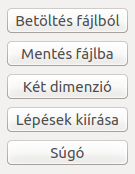
\includegraphics[width=4cm]{pics/gui/menu} \\
{\footnotesize Az alkalmazás menüje}
\end{center}
\paragraph{}
Az alappontokat automatikusan felosztással, és manuálisan egyenként is meg lehet adni. Erre a főképernyő felső részében van lehetőség, ahol fülek segítségével választható ki. A fülek alatt találhatóak a bemeneti mezők, melyekben a szükséges információkat tudjuk megadni. \\
\begin{tabular}{cc}
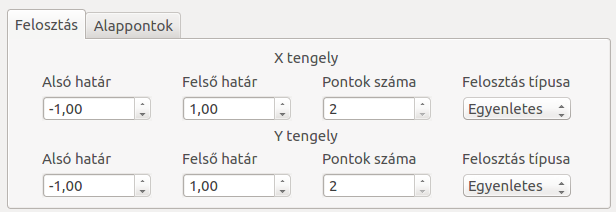
\includegraphics[width=7cm]{pics/gui/partition1} & 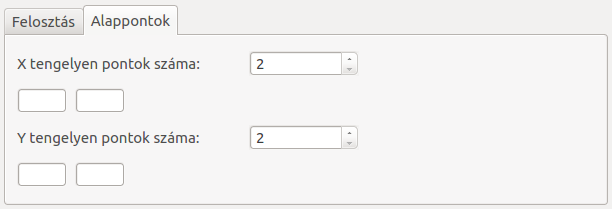
\includegraphics[width=7cm]{pics/gui/partition2} \\
{\footnotesize A két változóhoz tartozó intervallumok} & {\footnotesize Az alappontok manuális megadása} 
\end{tabular}

\subsection{Program felépítése}
\paragraph{}
A programot az MVC (modell - nézet - kontroller) architektúrában valósítjuk meg. A megjelenítésért felelős osztályok a View névtérben találhatóak, feladatuk a felhasználóval való kommunikáció, a bemeneti mezők megjelenítése, valamint a függvények vizualizációjának megjelenítése. A Model névtérben találhatóak a program logikáját tartalmazó osztályok, két névtérben (Parseval és Interpolation) a függvény kiértékeléshez és interpolációhoz szükségesek, valamint egy főosztály hangolja össze ezen részek működését. A Controller névtérben a nézet és modell közötti kommunikációt létrehozó osztály található. Feladata a felhasználói interakciók elküldése a modellnek, valamint a nézet frissítése a modell változásai alapján.
\begin{center}
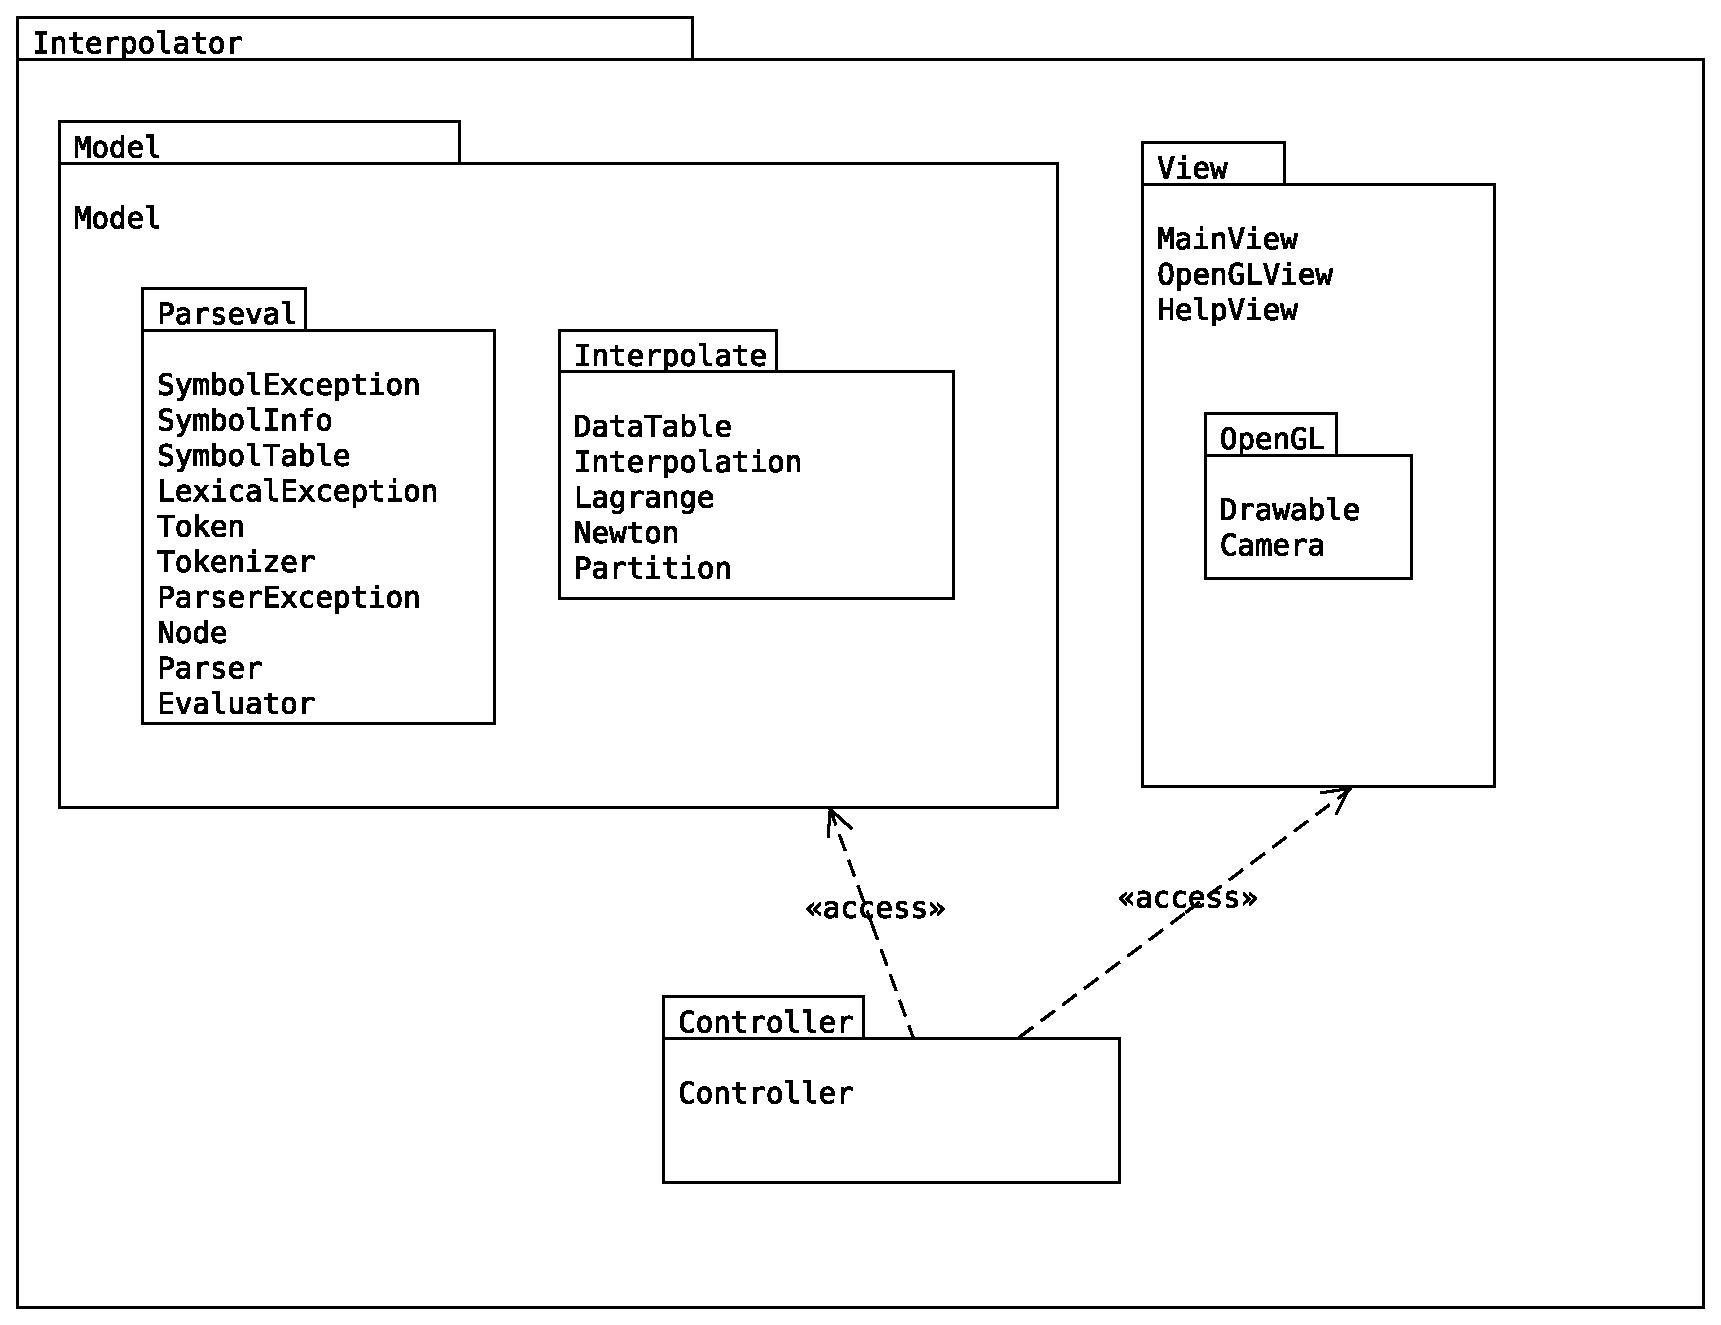
\includegraphics[width=14cm]{pics/uml/package}\\
{\footnotesize Az névterek kapcsolata}
\end{center}
\newpage

\section{Megvalósítás}
\subsection{Fázisok}
\subsubsection{Függvény elemző}
\subsubsection{Háromdimenziós megjelenítés}
\subsubsection{Interpolációs polinom előállítása}
\subsubsection{Grafikus felület elkészítése}
\subsubsection{Használhatóság könnyítése}
\subsubsection{Funkcionalitás bővítése}

\subsection{Az osztályok}
Az objektumorientált programozás módszertanát szem előtt tartva, minden metódust, adattagot osztályokba szervezve tárolunk. A programban számos osztály található, a közöttük lévő kapcsolatok az alábbi ábrán láthatóak.
\begin{center}
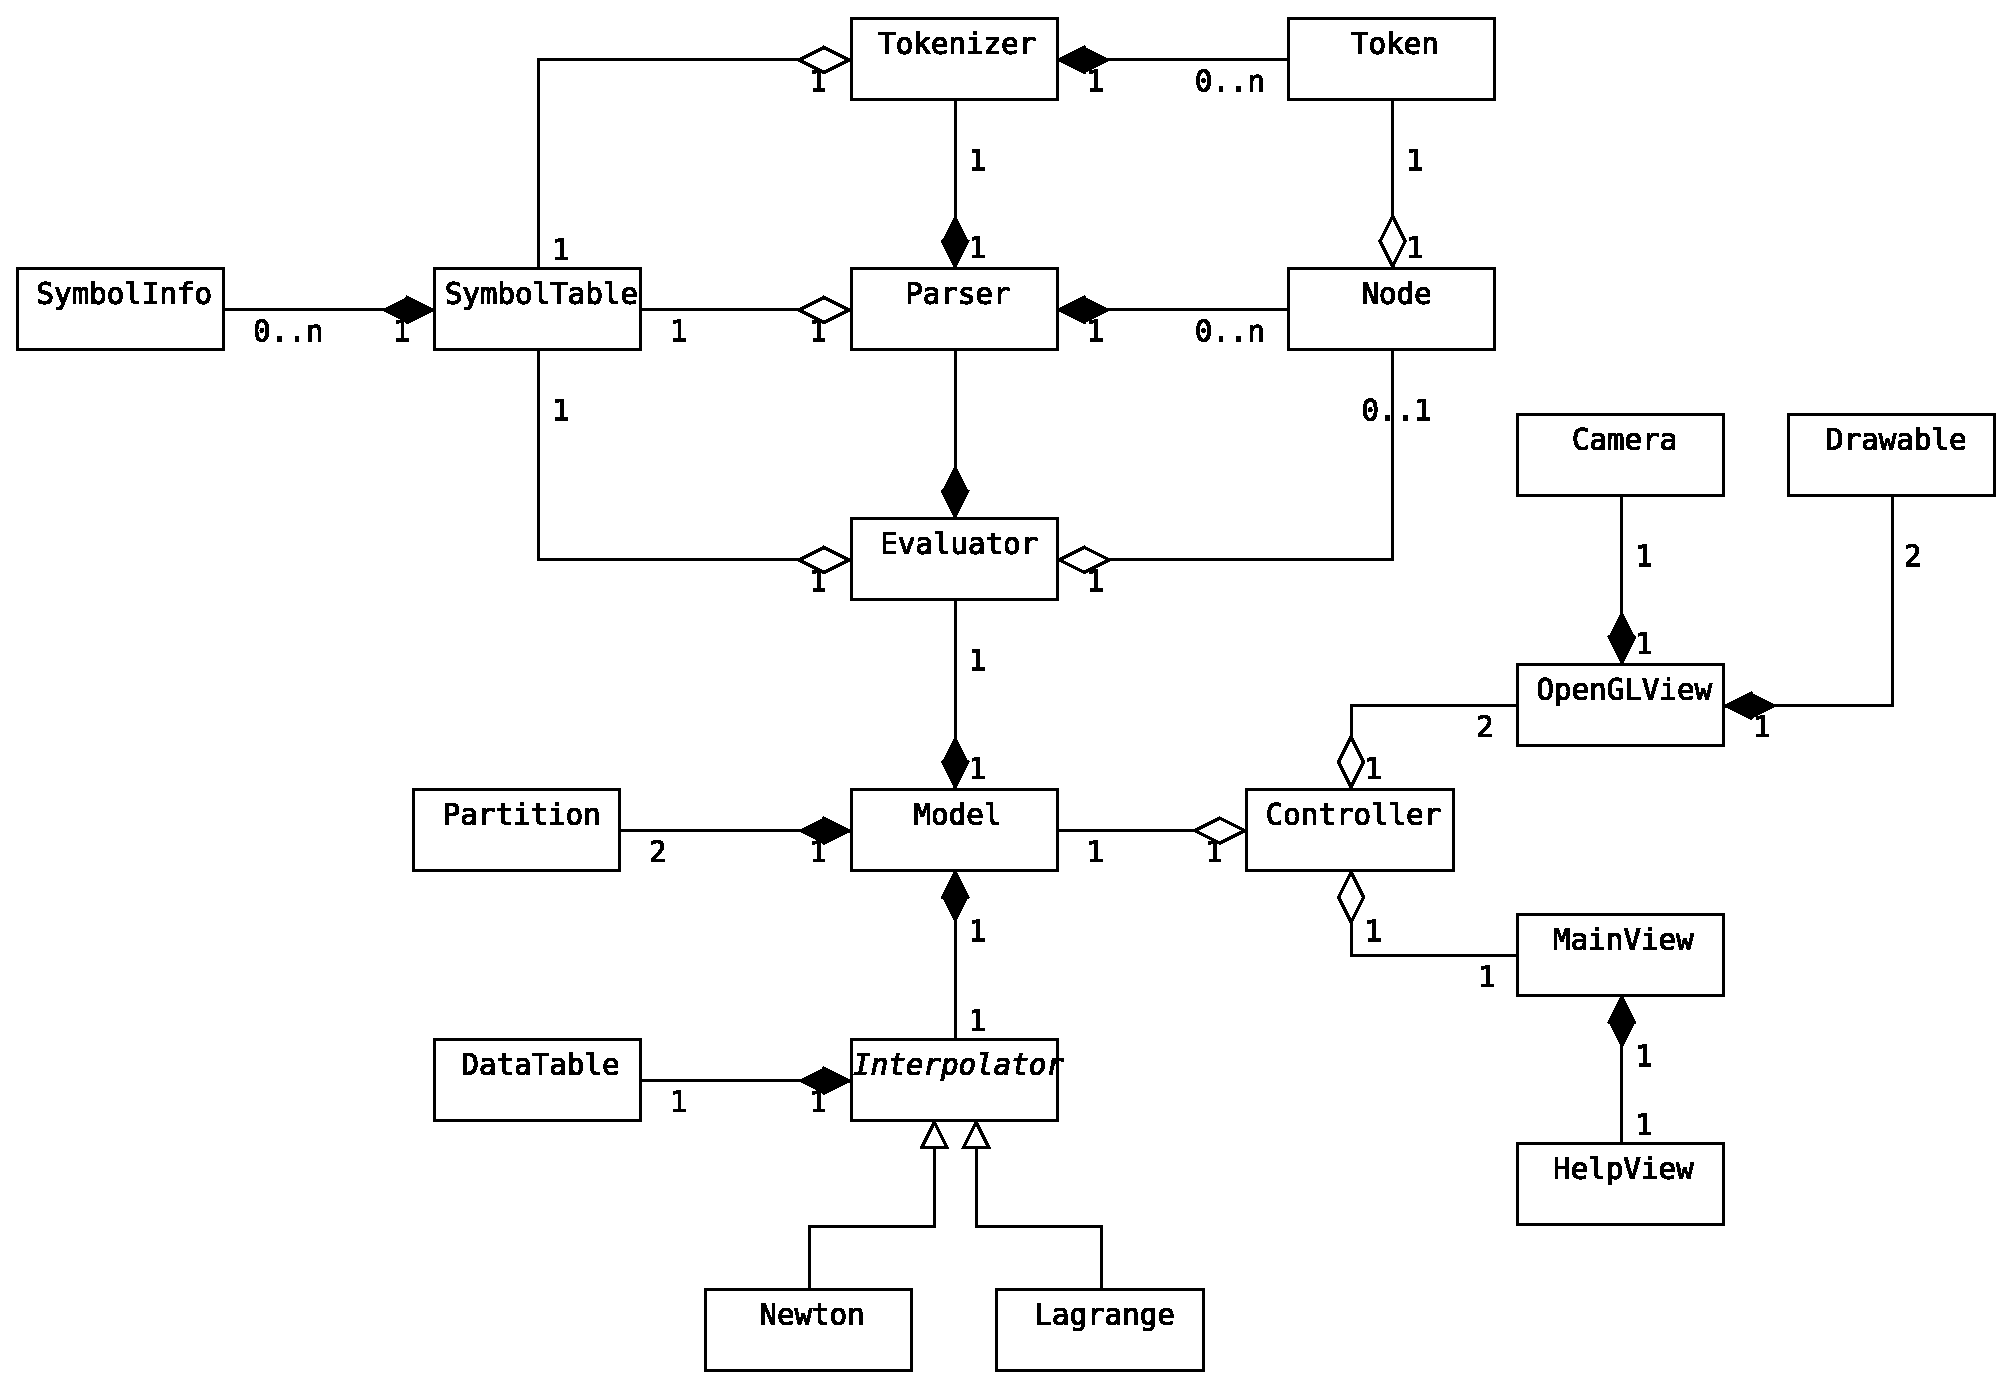
\includegraphics[width=14cm]{pics/uml/classes}\\
{\footnotesize Az osztályok kapcsolata}
\end{center}
\paragraph{}
A jobb átláthatóság érdekében az osztályok részletezése lentebb található, a diagram mellett egy rövid leírás és fontosabb metódusok bemutatása olvasható.

\subsubsection{Model névtér}
\paragraph{}
Az összes osztály, mely a program logikáját tartalmazza ebben a névtérben található. Két alnévtér található benne, az Interpolation és a Parseval, melyek teljesen elkülönülő feladatokat látnak el. Az első az interpolációt végzi, míg a második a matematikai függvények elemzését és kiértékelését.

\paragraph{SymbolException osztály}
Célja a SymbolTable osztály publikus metódusaiban keletkező hibák jelzése. Ősosztálya a QException osztály, így biztosítva van, hogy a kivétel szálbiztos. Pontosabb hibajelzés érdekében a konstruktorában megadható szöveges információ, mely egy privát adattagban tárolódik. A felülírt what() függvény segítségével kérdezhetjük le.
\begin{center}
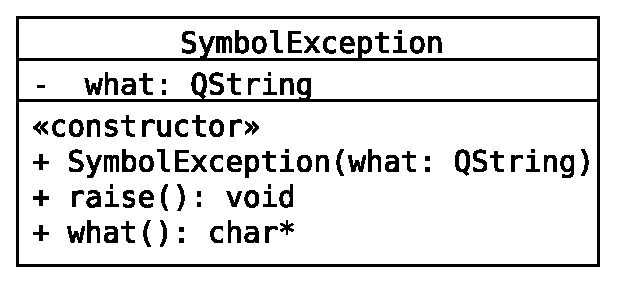
\includegraphics[width=6cm]{pics/uml/SymbolException}
\end{center}

\paragraph{SymbolInfo osztály}
A szimbólumokhoz fontos információk tartoznak, a SymbolInfo osztály feladata, hogy ezeket együttesen tárolja. A szimbólum neve, reguláris kifejezése, paraméter száma, bináris függvény esetén asszociativitása, precedenciája, illetve a kiszámításhoz szükséges függvény a konstruktorban megadott értékkel inicializálódik. A getterek segítségével kérdezhetjük le a szükséges információt, hatékonyság céljából mindegyik metódus egy konstans referenciával tér vissza, így nem történik másolás.
\begin{center}
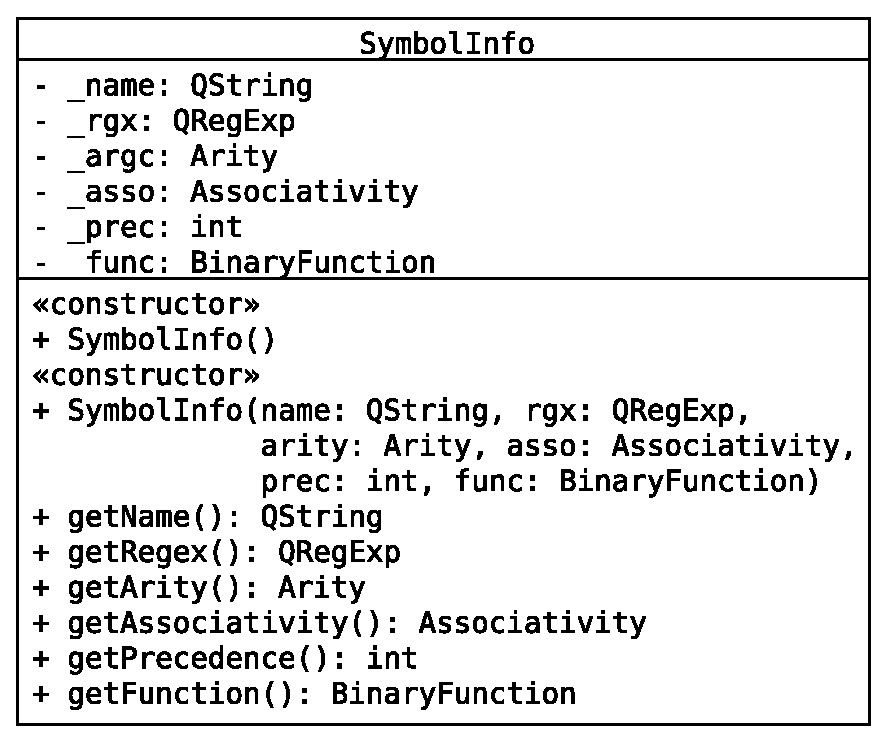
\includegraphics[width=8cm]{pics/uml/SymbolInfo}
\end{center}

\paragraph{SymbolTable osztály}
A szimbólumok rendszerett tárolására szolgál a SymbolTable osztály, mely a singleton tervezési mintát megvalósítva biztosítja, hogy a programban mindenhol ugyanazok a szimbólumok legyenek elérhetőek. A szimbólumok azonosítója a nevük, így feltétel, hogy ne szerepelhessen két szimbólum azonos névvel. Bejárást egy belső osztály, const\_iterator, teszi lehetővé. Biztosítja a gyorsaságot a másolás elkerülésével, azzal a feltétellel, hogy nem változtathatjuk az adatokat.
\begin{center}
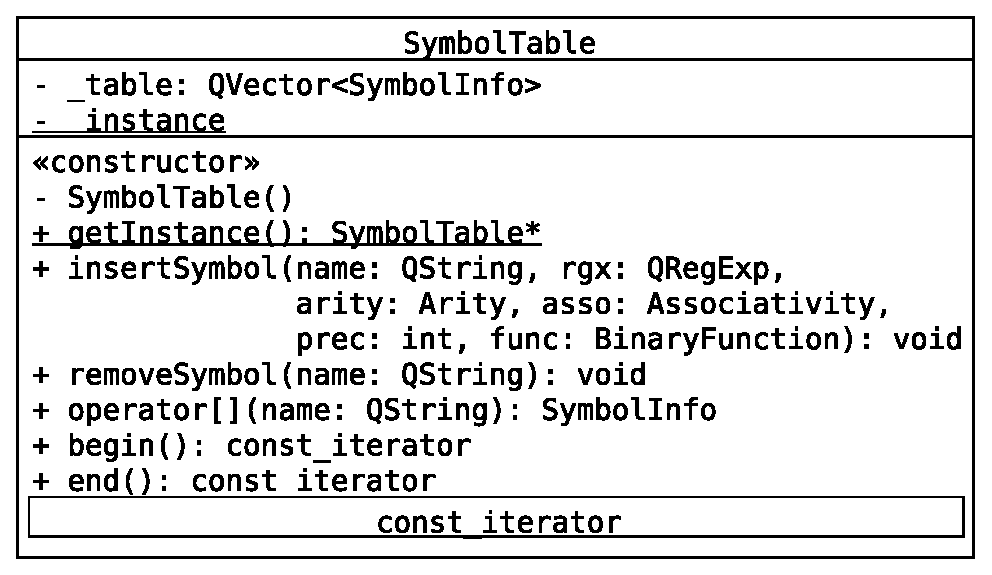
\includegraphics[width=10cm]{pics/uml/SymbolTable}
\end{center}
\begin{itemize}
\item A getInstance osztályszintű függvény segítségével kapjuk meg az osztály egyetlen példányát. Az értékadás operátor és másoló konstruktor törlésre került, a singleton tulajdonság miatt. 
\item Az insertSymbol metódus először megnézi, hogy létezik-e már szimbólum a megadott névvel a táblában, ha nem akkor beilleszti az új szimbólumot, ha már volt ilyen nevű, akkor pedig SymbolException kivételt dob.
\item Az operator[] név alapján keresi meg a szimbólumot, amennyiben létezik. Ha nem létezik a szimbólum, akkor SymbolException kivétel keletkezik.
\item Meglévő szimbólumot a removeSymbol segítségével, név alapján tudunk eltávolítani. Ha nem létezik szimbólum a megadott névvel, akkor SymbolException kivételt dob.
\end{itemize}

\paragraph{LexicalException osztály}
A LexicalException osztály célja, hogy jelezze a lexikális elemzés közben fellépők hibákat. Ősosztálya a QException osztály, így biztosítva van, hogy a kivétel szálbiztos. Pontosabb hibajelzés érdekében a konstruktorában megadható szöveges információ, mely egy privát adattagban tárolódik. A felülírt what() függvény segítségével kérdezhetjük le.
\begin{center}
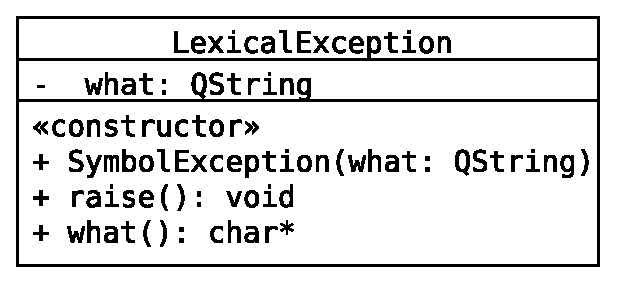
\includegraphics[width=6cm]{pics/uml/LexicalException}
\end{center}

\paragraph{Token osztály}
A feldolgozás első lépése, hogy a bemenetet szimbólumokra bontsuk. Mivel a szimbólumokat a nevük alapján tudjuk azonosítani, így elegendő azt eltárolni. A változók és számok esetén a szemantikus értéket is meg kell őriznünk, hogy később be tudjuk helyettesíteni az értékét. Példányosításkor a konstruktorban megtudjuk adni ezt a két információt, az adattagok ezekkel az értékekkel inicializálódnak.
\begin{center}
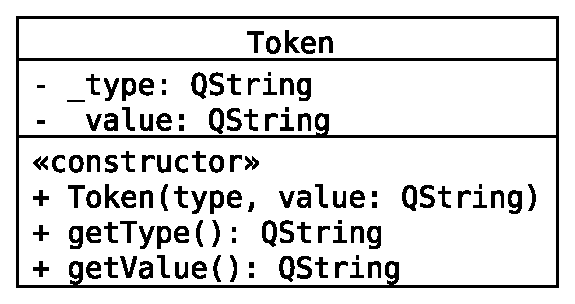
\includegraphics[width=6cm]{pics/uml/Token}
\end{center}

\paragraph{Tokenizer osztály}
A Tokenizer osztály az függvény szöveges megadása után, a szimbólumtábla segítségével, tokenekre bontja a bemenetet. A jobb párhuzamosság elérése céljából, bontja fel azonnal a bemenetet. Megpróbálja a bemenetet megfeleltetni valamelyik szimbólumnak, ha sikerül, akkor elmenti egy adattagba a kapott eredményt, és lépteti a bemenetet. Ha nem talál egyezést egyik szimbólum reguláris kifejezésére sem, akkor LexicalException kivétel dobásával jelzi azt.
\begin{center}
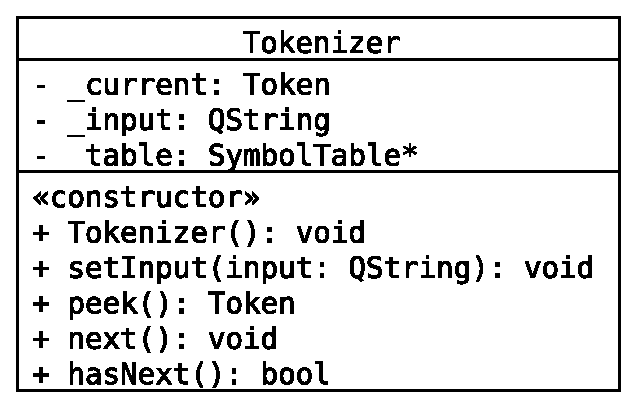
\includegraphics[width=6cm]{pics/uml/Tokenizer}
\end{center}
\begin{itemize}
\item A next metódus ismeri fel a következő szimbólumot. Végig iterál a SymbolTable osztály egyetlen példányán, és ha talál egyezést, akkor azt a \_current változóban tárolja. Amennyiben végigért a táblán, de nem talált egyezést, akkor egy LexicalException kivétel dobásával jelzi azt, megadva, hogy hol akadt el a bemeneten.
\item A peek metódus segítségével kérdezhetjük le a jelenlegi Token-t.
\end{itemize}

\paragraph{ParserException osztály}
Az osztály célja, hogy a szintakszis fa építése közben keletkező hibákat jelezze. Ősosztálya a QException osztály, így biztosítva van, hogy a kivétel szálbiztos. Pontosabb hibajelzés érdekében a konstruktorában megadható szöveges információ, mely egy privát adattagban tárolódik. A felülírt what() függvény segítségével kérdezhetjük le.
\begin{center}
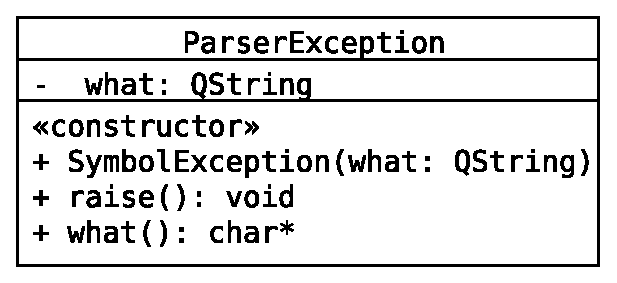
\includegraphics[width=6cm]{pics/uml/ParserException}
\end{center}

\paragraph{Node osztály}
Láncolt, bináris fa építőköve. Egy csúcsról tárolja a benne tárolt tokent, valamint a két gyerekről egy-egy mutatót. Így fentről-lefelé mélységi bejárással gyorsan végig tudunk menni a gráfon.
\begin{center}
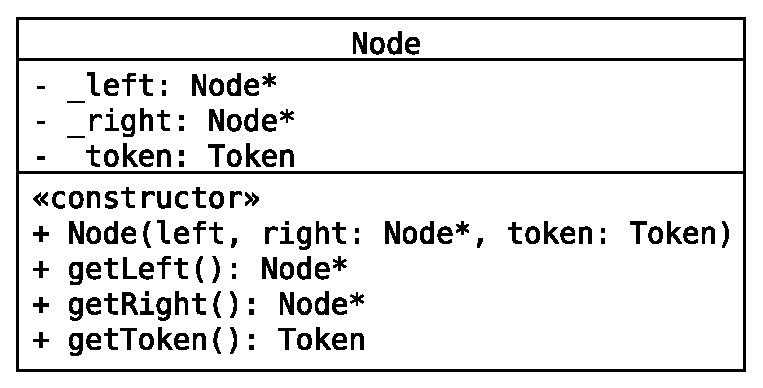
\includegraphics[width=6cm]{pics/uml/Node}
\end{center}

\paragraph{Parser osztály}
A precedecia elemző implementációja. Feladata felismerni az egyszerű és összetett kifejezeséket és felépíteni belőlük a szintakszis fát. A lexikális elemzővel folyamatos összeköttetésben áll, ő mondja meg, hogy mikor lépjen a következő szimbólumra. Ennek a következménye, hogy a szintakszisfát lineáris időben előtudja állítani.
\begin{center}
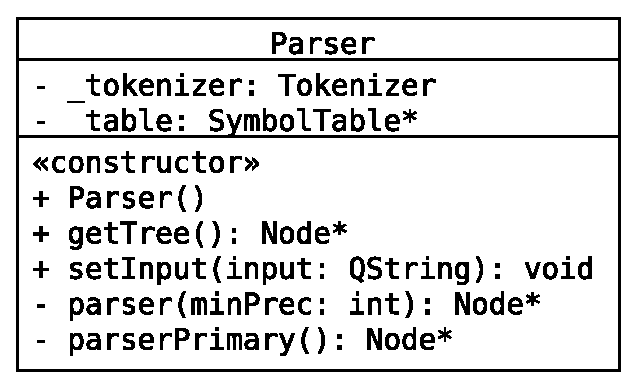
\includegraphics[width=6cm]{pics/uml/Parser}
\end{center}
\begin{itemize}
\item A parsePrimary metódus ismeri fel az elemi kifejezéseket, melyek lehetnek számok, változók, függvények vagy zárójelben álló összetett kifejezések. Kivétel keletkezik, ha a előjel után nem áll kifejezés, ha nem megfelelő a zárójelezés, ha hiányzik a függvény paramétere, illetve ha bináris operátoron áll az input.
\item A parse függvény az elemi kifejezésekből épít fel összetett kifejezéseket, ügyelve arra, hogy a műveletek megfelelő sorrendben következzenek egymás után. Ehhez felhasználja a szimbólumok precedenciáját és asszociativitását. Kivételt dob, ha nem áll két elemi kifejezés között bináris operátor.
\item A getTree metódus indítja el a teljes rekurzív folyamatot, és visszatérési értéke a szintakszis fa gyökerére mutató pointer. 
\end{itemize}

\paragraph{Evaluator osztály}
A precedencia elemző által előálított fát megadott pontokban ki kell számolni. Ehhez a gyökérből elindulva, postorder mélységi bejárást használva végigmegy a fán, és a változók helyére a szemantikus érték alapján a megfelelő értéket helyettesíti, illetve számok esetén magát a szemantikus értéket helyettesíti be. A számolás költségének csökkentése érdekében egy gyorsítótárral rendelkezik, mely az x,y értékpárokhoz hozzárendeli a függvény értékét, így a következő alkalommal nem kell kiszámolni, elegendő csak innen kiolvasni.
\begin{center}
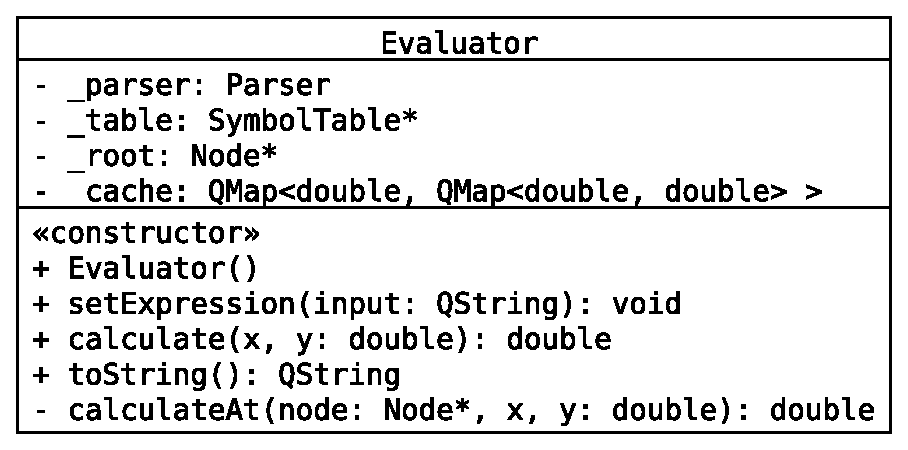
\includegraphics[width=10cm]{pics/uml/Evaluator}
\end{center}
\begin{itemize}
\item A calculate függvény először megnézi, hogy a \_cache-ben található-e érték az x,y párhoz, ha igen akkor visszaadja azt. Amennyiben még nincs érték hozzá, akkor a calculateAt függvény segítségével kiszámolja a gyökérben a függvény értékét, majd eltárolja a \_cache-ben.
\item A calculateAt metódus valósítja meg a mélységi bejárást a node csúcsból. Rekurzívan addig megy le a fában, amíg levelet nem talál, és közben folyamatosan elvégzi az adott műveletet. Függvények és operátorok esetén a szimbólumtáblából kérdezi le az adott műveletet.
\end{itemize}

\paragraph{DataTable osztály}
Az alappontokat sokszor az indexük alapján használjuk az interpoláció során, az osztály levehető teszi, hogy tároljuk, és az index alapján elérjük az alappontokat, és az ott felvett értékeket. Az alappontok növekvő sorrendben vannak tárolva, így a beszúrás lineáris idejű. Mivel feltétel, hogy a rács minden pontjában meglegyen adva a függvény értéke, ezért beszúráskor egyből egy sort vagy oszlopot tesz be.
\begin{center}
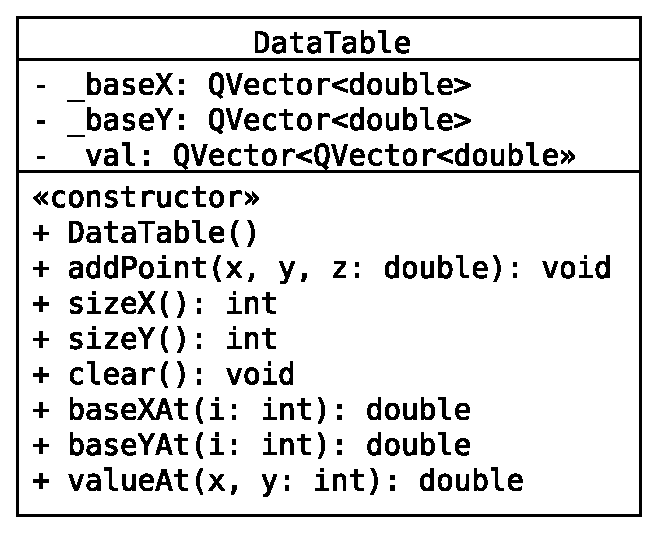
\includegraphics[width=7cm]{pics/uml/DataTable}
\end{center}
\begin{itemize}
\item Az addPoint metódus először megnézi, hogy az adott x, y értékekhez tartozik-e oszlop és sor, ha bármelyik hiányzik, akkor beszúr egyet neki. Ezután a mátrix megfelelő cellájába behelyezi az értéket.
\item A többi függvény segítséget nyújt index alapú lekérdezéshez.
\end{itemize}

\paragraph{Interpolation osztály}
Egy absztrakt osztály, mely segítséget nyújt ahhoz, hogy a megvalósítást többféle, különböző módon valósítsuk meg. Az alappontokat kezeli, de a kiszámítás már egy tisztán virtuális függvény segítségével van megvalósítva. Ennek következménye, hogy az osztályt nem tudjuk példányosítani. Származtatáskor pedig felül kell írnunk, és itt tudjuk kiszámolni az eredményt.
\begin{center}
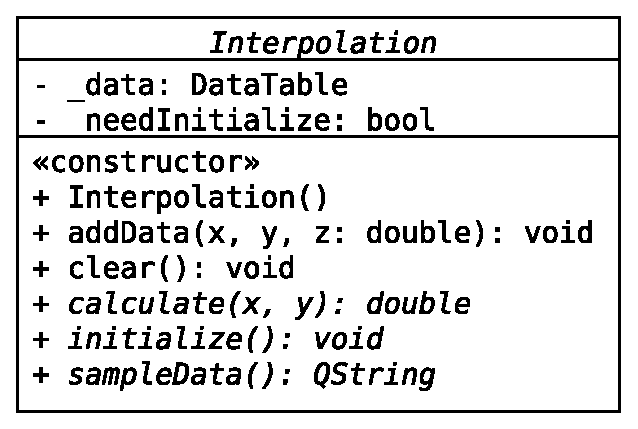
\includegraphics[width=7cm]{pics/uml/Interpolation}
\end{center}

\paragraph{Lagrange osztály}
A polinom interpoláció Lagrange alakját használva készíti el a függvény közelítését. Mivel az Interpolation-ből származtatott osztály, így az alappontok kezelésével már nem kell foglalkoznia, csak a polinom előállításával és kiszámításával. Első lépésben előállítja a Lagrange alappolinomokat mindkét változóra, a calculate függvényben pedig kiértékeli őket az adott pontban.
\begin{center}
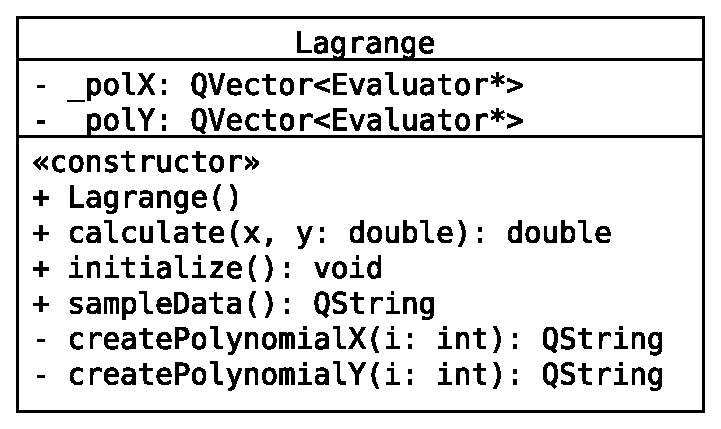
\includegraphics[width=7cm]{pics/uml/Lagrange}
\end{center}
\begin{itemize}
\item A createPolynomialX és createPolynomialY metódusok előállítanak egy darab alappolinomot, mely a paraméterben megadott alapponthoz tartozik.
\item Az initialize függvény az összes alappontra elkészíti az alappolinomokat, a két createPolynomial segédfüggvény segítségével.
\item A calculate metódus az alappolinomokat kiértékeli a pontban, megszorozza a megfelelő függvényértékkel, majd összeadja őket.
\end{itemize}

\paragraph{Newton osztály}
A Newton-alakú interpolációt használva, az osztott differenciák segítségével készíti el a közelítést. Az Interpolation osztályból származtatott, így az alappontok kezelésével nem kell foglalkoznia. A differenciák előállítása után, a Horner algoritmus segítségével értékeli ki a polinomot az adott pontban.
\begin{center}
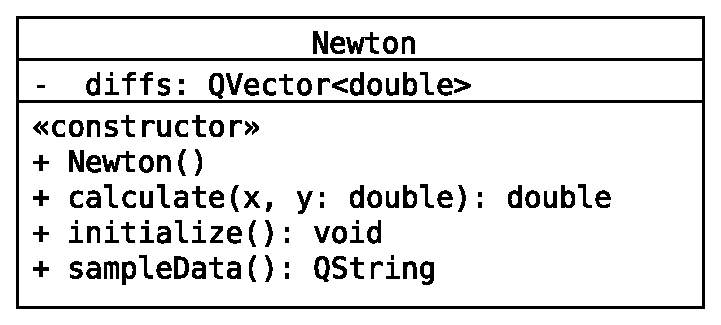
\includegraphics[width=7cm]{pics/uml/Newton}
\end{center}
\begin{itemize}
\item Az initialize metódus számolja ki a pontokhoz tartozó osztott differenciákat, ezek a \_diffs vektorban tárolódnak.
\item A calculate függvény a Horner algoritmus segítségével értékeli ki a polinomot.
\end{itemize}

\paragraph{Partition osztály}
Egy intervallum felosztását tárolja. Automatikusan előtudja állítani a pontokat, egyenletesen elosztva, vagy a Csebisev polinomok gyökeinek transzformációjával. Manuálisan is megadható a kívánt alappontok halmaza.
\begin{center}
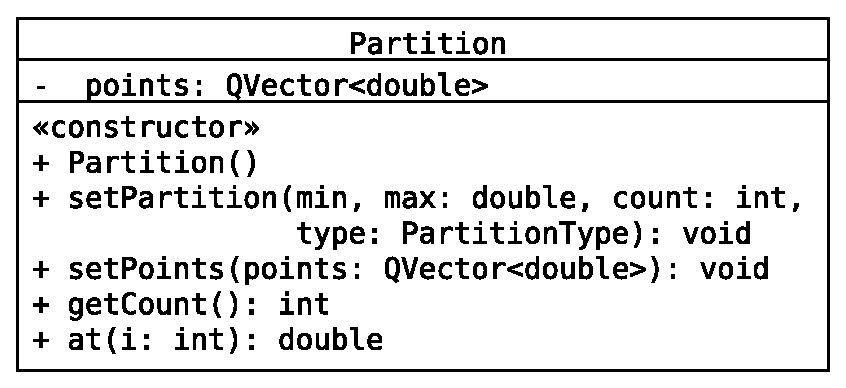
\includegraphics[width=7cm]{pics/uml/Partition}
\end{center}
\begin{itemize}
\item A setPartition függvény a típus alapján generálja ki a felosztást, ezzel megsegítve a felhasználó munkáját.
\end{itemize}

\paragraph{Model osztály}
A Model feladata, hogy összehangolja a különböző modulokat, elvégezze a szükséges számításokat és jelezze a nézeteknak a megjelenítendő adatokat. Lehetőséget biztosít arra, hogy a lépéseket megjelenjenek a felhasználó számára. A nézettel a kontroller osztályon keresztül, szignálokkal kommunikál, mely a QObject osztályból való származtatással lehetséges.
\begin{center}
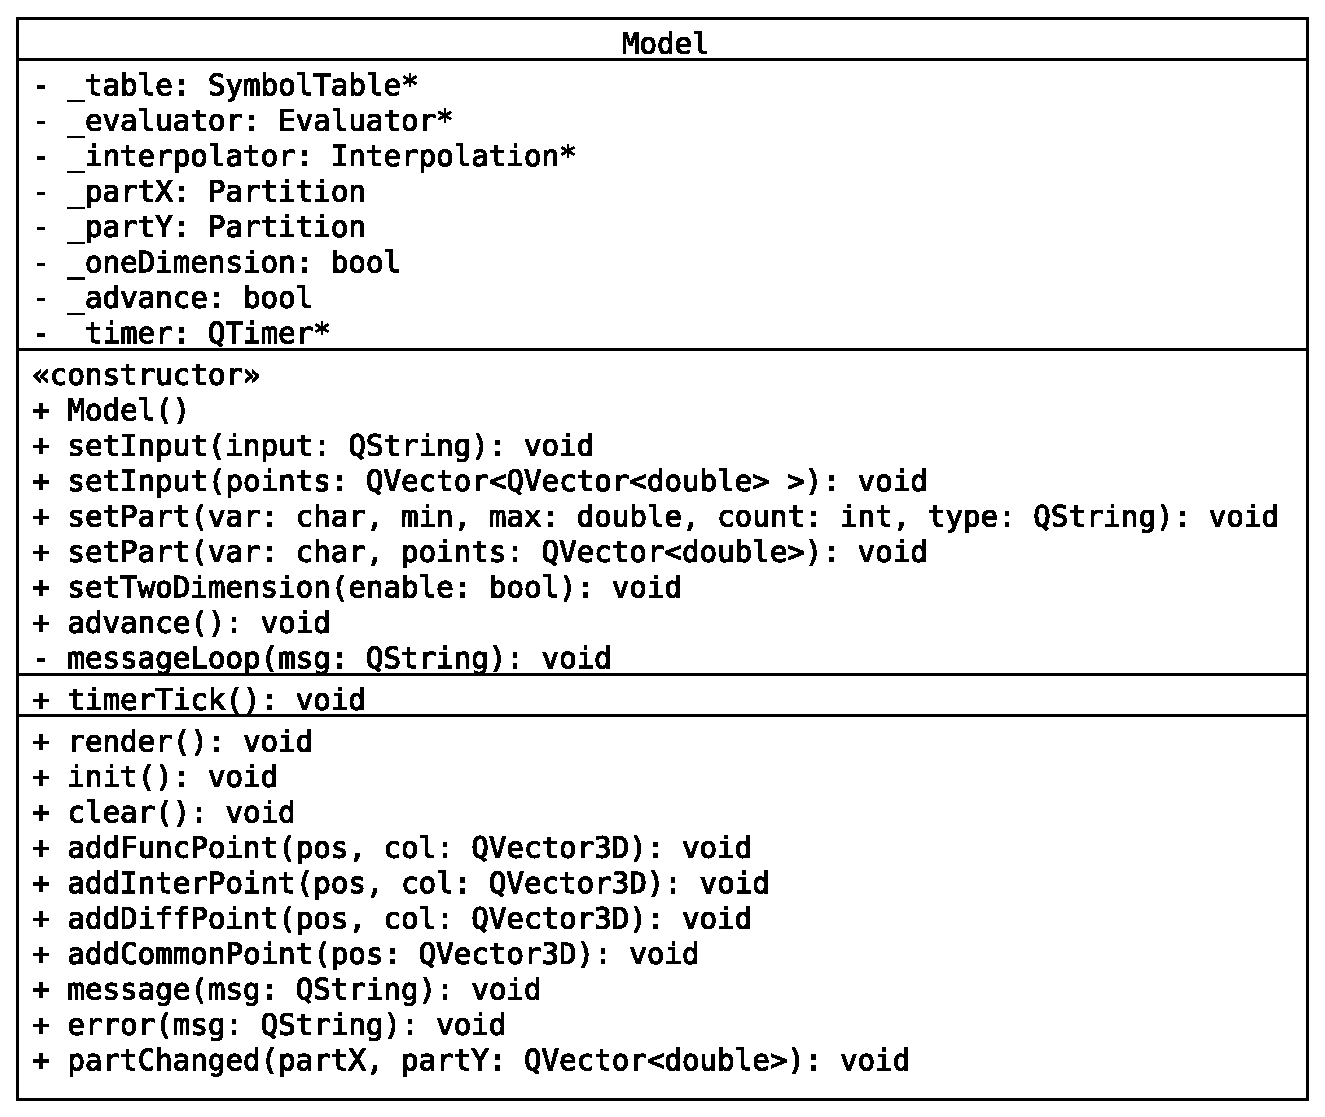
\includegraphics[width=10cm]{pics/uml/Model}
\end{center}
\begin{itemize}
\item A setPart függvények segítségével lehet beállítani az adott változóhoz tartozó alappontokat. A felüldefiniálás segítségével támogatja a manuális és az automatikus beállítást is.
\item A setInput metódus meghívásával kezdődik el a fő megjelenítési folyamat, ami két részre oszlik, és több lépésből áll.
\item Függvény megadása esetén:
	\begin{itemize}
		\item A bemenetből, ha lehetséges, akkor előállítja a szintakszis fát.
		\item A függvényt az alappontokban kiértékeli, és ez alapján beállítja az interpoláció alappontjait és értékeit.
		\item Előállítja az interpolációs polinomot.
		\item Véges sok pontban kiértékeli a függvényt és a közelítést, és elküldi az adatokat a megjelenítőnek.
		\item Elküldi a jelet a nézetnek, hogy elkezdheti az inicializációt és a megjelenítést.
	\end{itemize}
\item Függvény értékek esetén:
	\begin{itemize}
		\item Beállítja az interpolációhoz.
		\item Előállítja az interpolációs polinomot.
		\item Véges sok pontban kiértékeli a közelítést és elküldi az adatokat a megjelenítőnek.
		\item Elküldi a jelet a nézetnek, hogy elkezdheti az inicializációt és a megjelenítést.
	\end{itemize}
\item Különböző típusú információt a message és error szignálok segítségével közöl, melyek paraméterében található az üzenet. A message a lépések megjelenítéséhez használt, míg az error a feldolgozás alatt keletkezett hibák jelzésére szolgál.
\end{itemize}

\subsubsection{Controller névtér}
A kontroller feladata, hogy vezérleje a többi egység működését, összeköttetést biztosít a nézetek és a modell között. 

\paragraph{Controller osztály}
Mivel a modell és a nézetek is szignálok segítégével jelzik a változásokat, így feladata ezeket kezelni. A szignálok kezeléséhez a QObject osztályból származik, és injektálás útján kapja meg az objektumokat, melyek szignáljaira rákapcsolja a megfelelő kezelőket. Mivel ő az, aki mindenki lát a rendszerben, így nincs szüksége szignálokra, függvényhívások segítségével hajt végre mindent.
\begin{center}
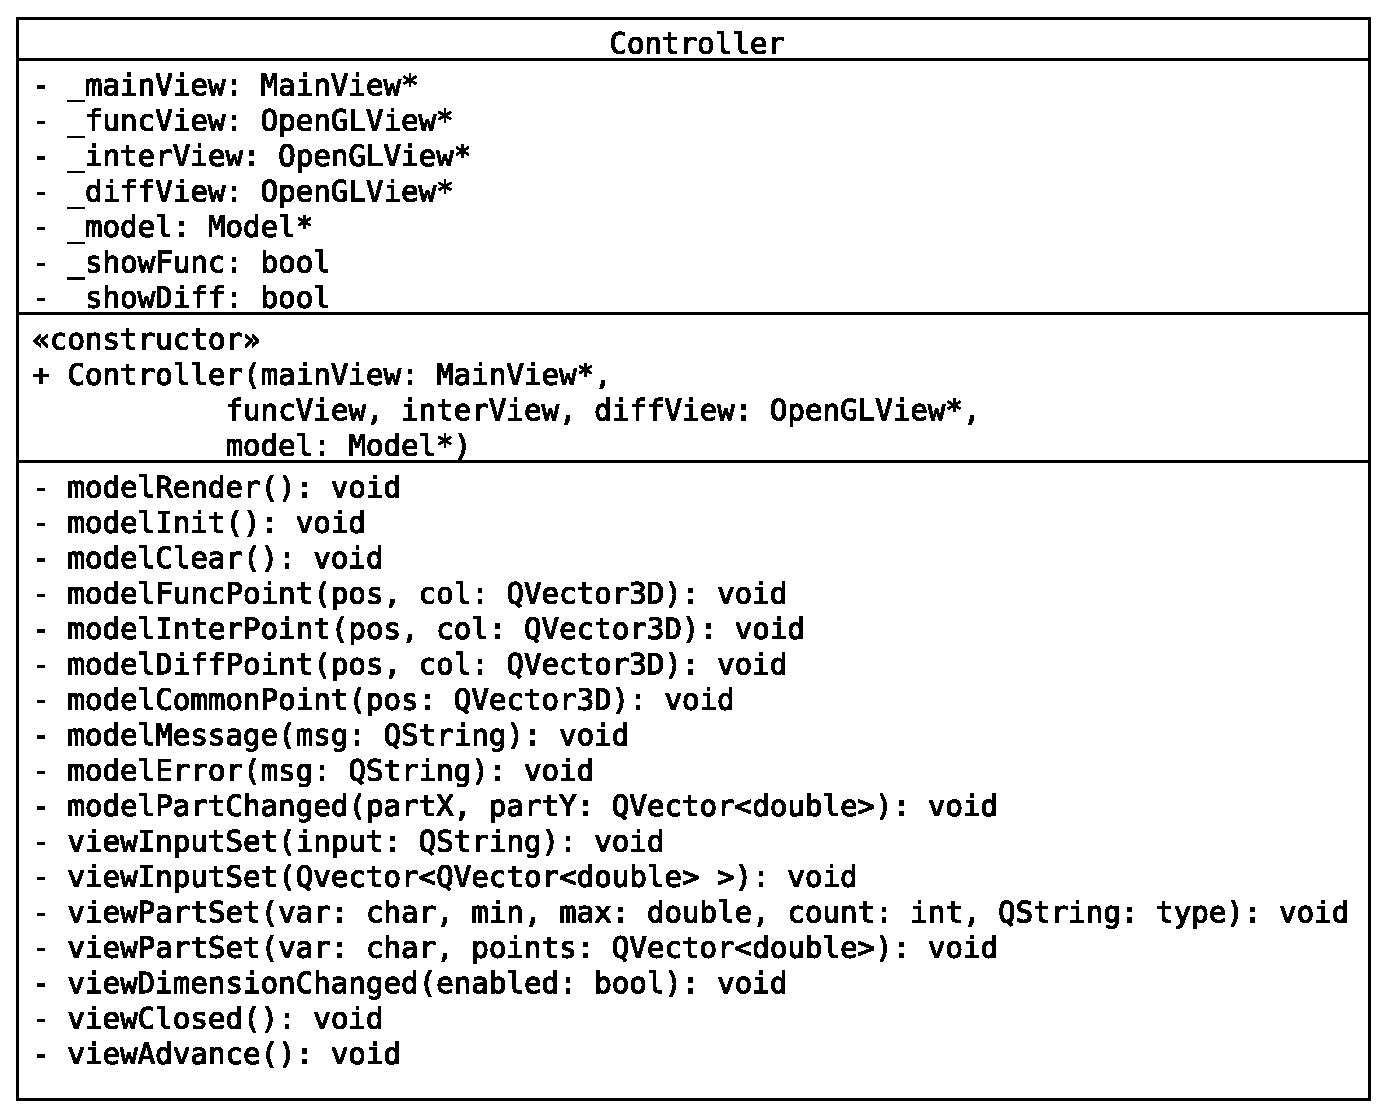
\includegraphics[width=10cm]{pics/uml/Controller}
\end{center}
\begin{itemize}
\item Minden kezelőjéhez tartozik egy azonos nevű szignál a megfelelő osztályban, ezzel könnyítve az átláthatóságot. Ezekben a függvényekben további hívja meg a megfelelő objektum megfelelő metódusát a kapott paraméterekkel.
\item Egyetlen kitüntetett feladata van, eldönteni, hogy meg kell-e jeleníteni a függvény nézetét is, vagy sem. Ez attól függ, hogy a modell küldött-e a nézetnek adatot, vagy sem.
\end{itemize}

\subsubsection{View névtér}
A felhasználóval való kommunikáció és információ közlés a nézetben található osztályok feladata. Egyéb segédosztályok is találhatóak benne, melyek a grafikus megjelenítéshez szükségesek.

\paragraph{Drawable osztály}
A célja egy grafikus alakzat tulajdonságainak beállítása és rendszerezése. Tárolja a pontok koordinátáját és színét a memóriában. Inicializáláskor lefoglalja az adatoknak szükséges területet a grafikus kártyán, majd miután felparaméterezte azt, át is másolja őket.
\begin{center}
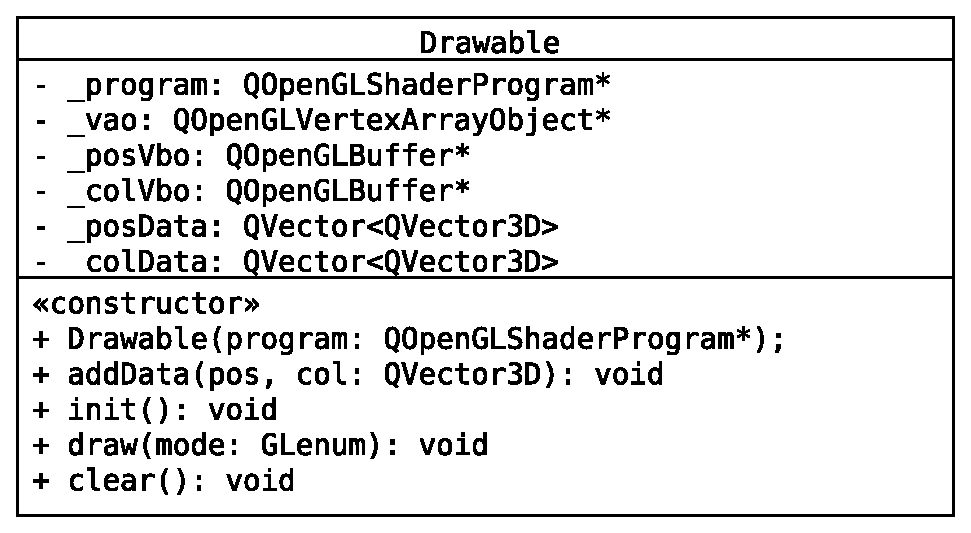
\includegraphics[width=7cm]{pics/uml/Drawable}
\end{center}
\begin{itemize}
\item A pontokat az addData függvény segítségével tudjuk megadni, ekkor még csak a memóriába kerülnek be az információk, csak az init függvény meghívásával másolódnak át. Így a teljes alakzatot egyben tudjuk kezelni.
\item A draw metódus rajzolja ki a tárolt objektumot a képernyőre, szükséges megadnunk a pontok összekötésének módját, a modell egyváltozós függvény esetén vonalakkal, kétváltozós esetén háromszögekkel dolgozik.
\end{itemize}

\paragraph{Camera osztály}
A térben elhelyezett kamera szerepét tölti be. Az osztályszintű metódusai a mátrixtranszformációk egyszerű használatát teszik lehetővé. A vertex transzformációhoz szükséges világ, nézet és vetítés mátrixokat is letudjuk kérdezni. A világban történő mozgást is a kamera eltolásával végezzük.
\begin{center}
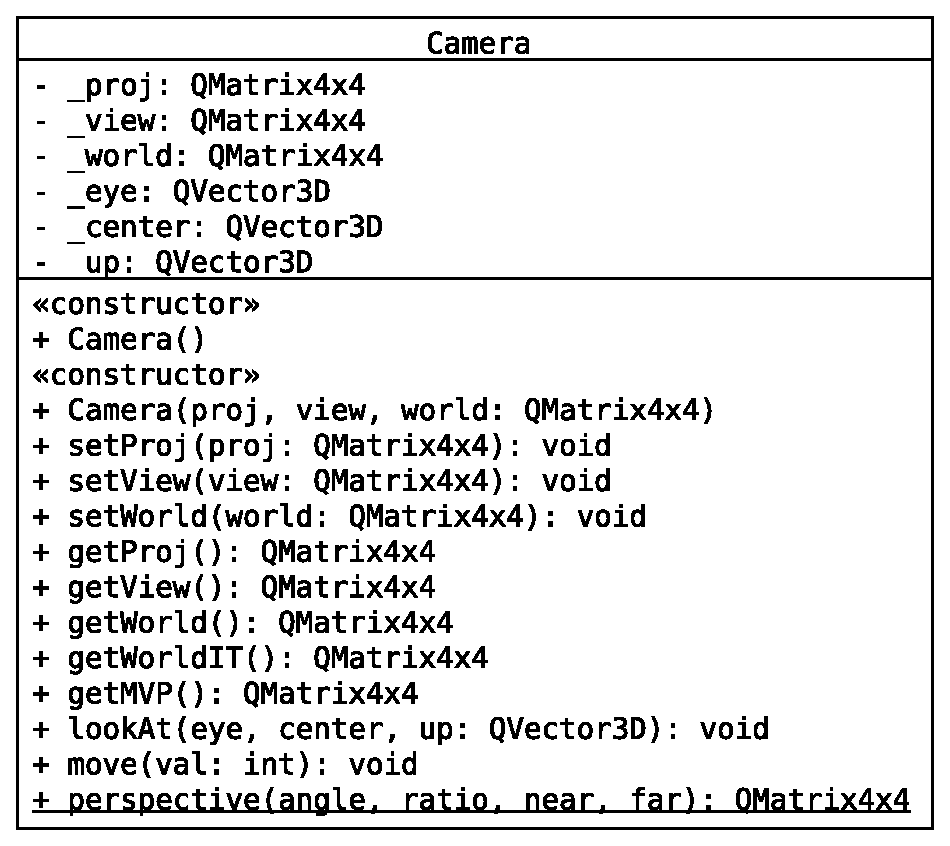
\includegraphics[width=7cm]{pics/uml/Camera}
\end{center}
\begin{itemize}
\item A lookAt függvény segítségével tudjuk megadni, hogy honnan melyik pontra nézünk. Szükséges még megadnunk a felfelé mutató irányt is.
\item A move metódussal tudjuk a kamerát közelíteni, illetve távolítani a középponthoz képest.
\end{itemize}

\paragraph{OpenGLView osztály}
Az osztály egy OpenGL támogatással rendelkező ablakot valósít meg, melyben megjelenik a függvény. A QOpenGLWidget osztályból származik, így a szükséges inicializációkat már nem kell elvégeznie. Egy beépített koordináta rendszerrel rendelkezik, illetve lehetőséget nyújt, hogy egy alakzat adatait is megadjuk.
\begin{center}
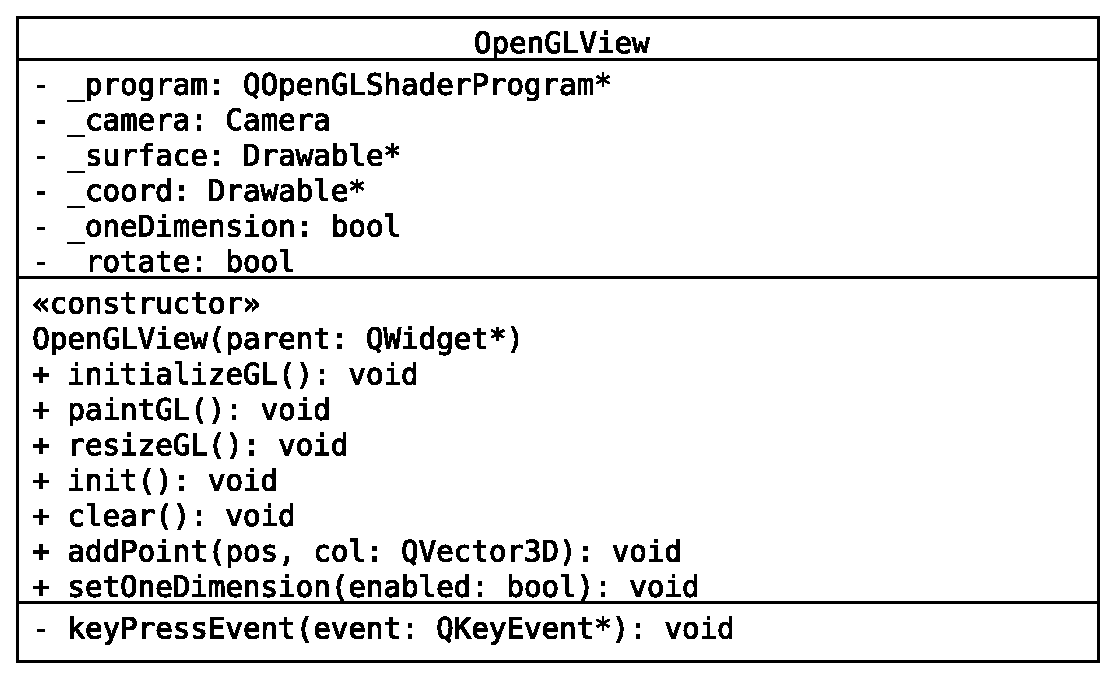
\includegraphics[width=7cm]{pics/uml/OpenGLView}
\end{center}
\begin{itemize}
\item Az initializeGL függvényben minden szükséges inicializációt elvégzünk, hogy a későbbiekben a kirajzolás folyamata minél gyorsabb legyen.
\item A paintGL függvényben történik a renderelés, törekedve a minél jobb teljesítményre, a függvény gyorsan végrehajtódik.
\end{itemize}

\paragraph{MainView osztály}
Feladata a felhasználóval való kommunikáció megvalósítása, illetve ha szükséges, az információk továbbítása a modell felé. A QWidget osztályból származik, így rendelkezik grafikus felülettel, melyen elhelyezett bemeneti mezők és nyomógombok segítségével tudja használni a programot.
\begin{center}
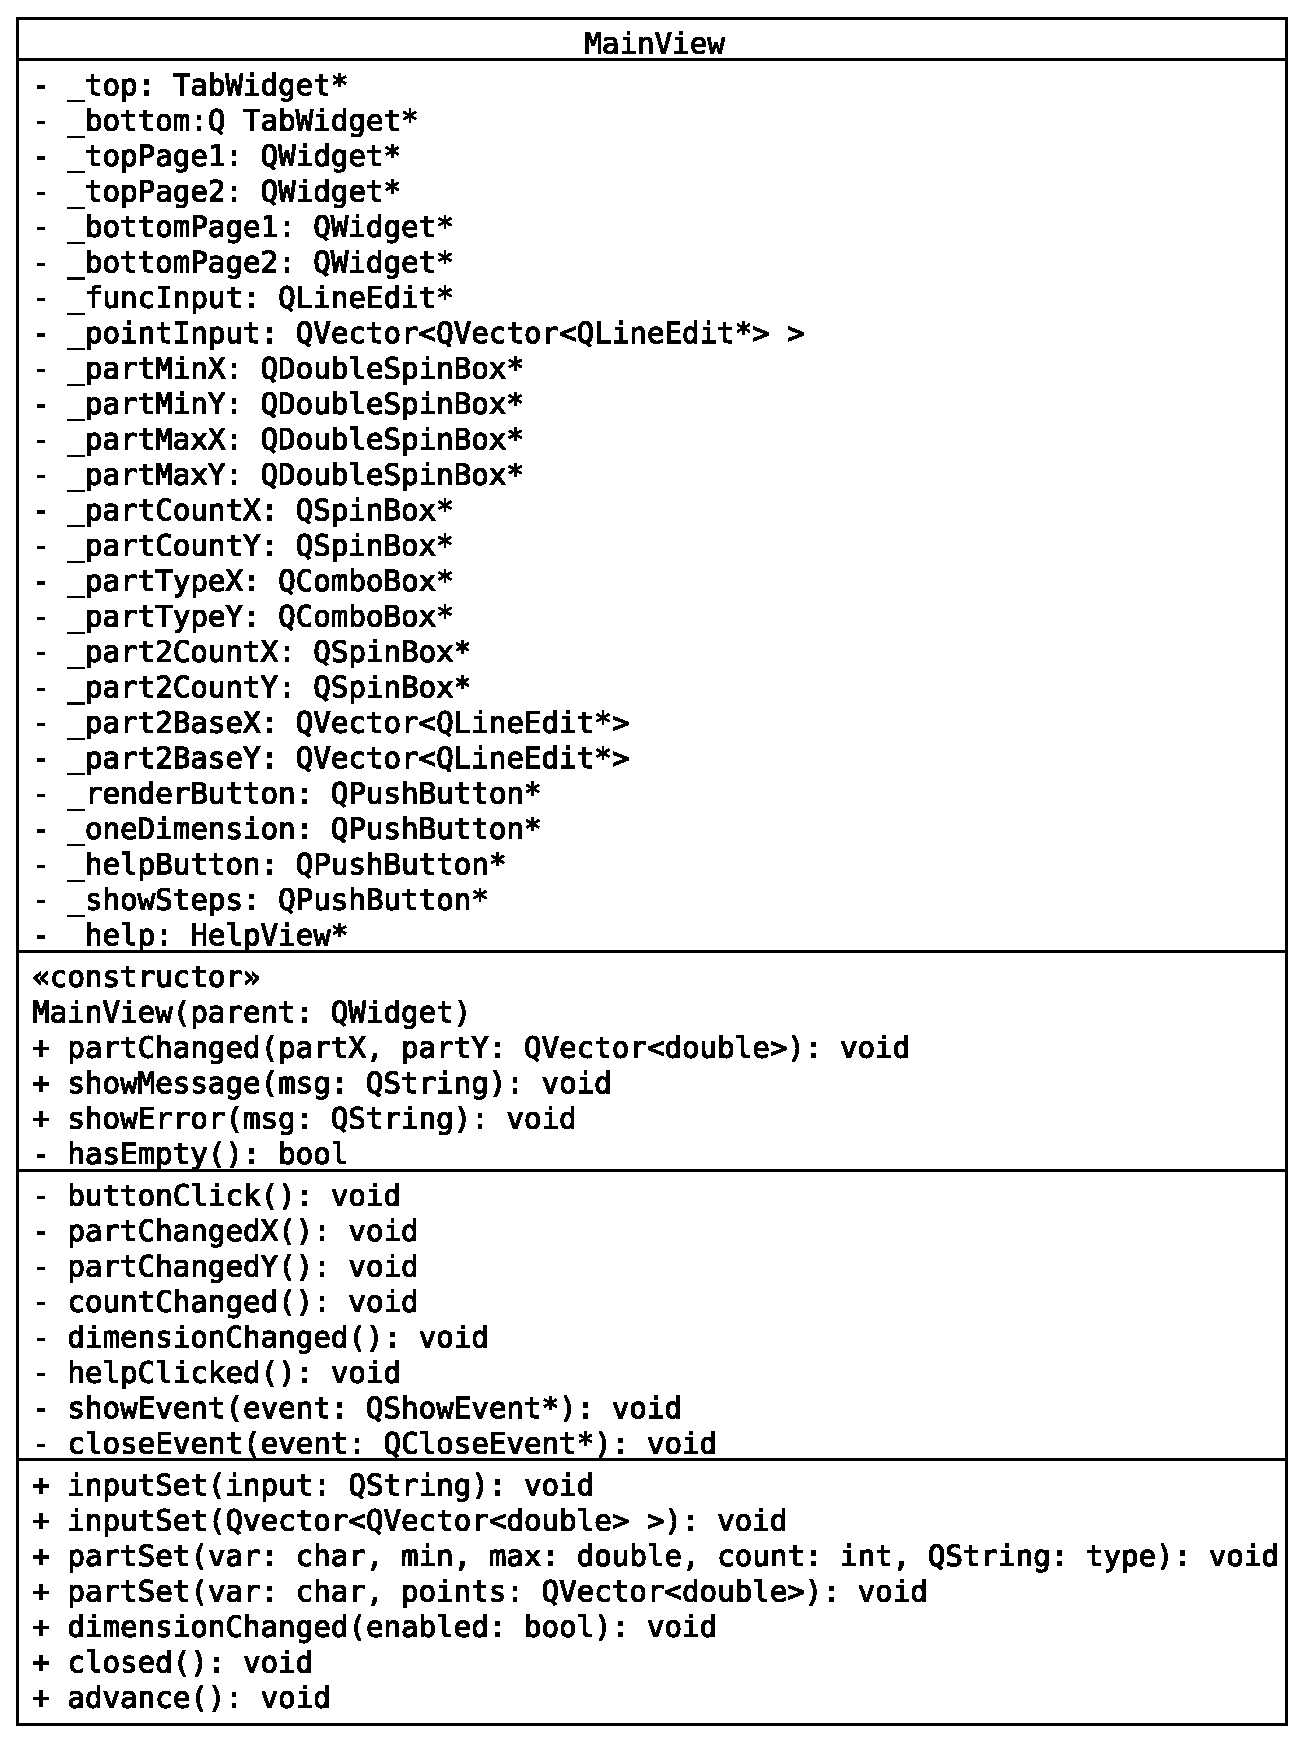
\includegraphics[width=10cm]{pics/uml/MainView}
\end{center}

\paragraph{HelpView osztály}
A súgó megjelenítésért felelős osztály, a QDialog osztályból származik, így amíg nem zárjuk be, nem tudjuk használni a bemeneti nézetet. Rendelkezik egy nyomógombbal, mely segítségével vissza tudunk térni. A különböző fülek alatt érhetjük el az egyes információkat.
\begin{center}
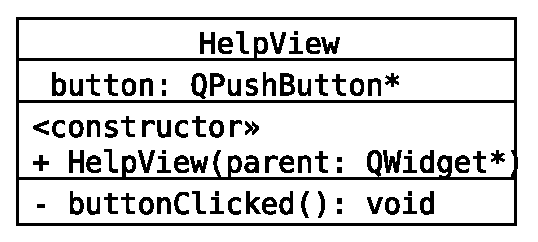
\includegraphics[width=5cm]{pics/uml/HelpView}
\end{center}

\section{Tesztelés}
A tesztelést két csoportban végeztem el. Először a modell fő funkcionalitásainak helyes működését teszteltem, utána pedig a végleges program használhatóságát.

\subsection{Egységtesztek}
\paragraph{}
A QtTest keretrendszer segítségével automatizált tesztelést valósítottam meg. Célja az, hogy a modell részkomponensei megfelelően működjenek, ezzel biztosítva, hogy a program is helyesen működjön.
\paragraph{}
A tesztek megtalálhatóak a test mappában, és az InterpolatorTest projekt használatával hajthatóak végre. Az alábbi tesztesetek kerültek megvalósításra:
\begin{itemize}
\item A szimbólumtáblába való beszúrás, eltávolítás és a táblából való lekérdezés.
\item A lexikális elemző működése helyes, illetve különböző hibás bemenetek esetén.
\item A függvény kiértékelő eredményének helyessége különböző függvények és több pontjában.
\item Az elkészített interpoláció átmegy az alappontokon a Newton- és Lagrange-alakban leírt függvények esetén is.
\end{itemize}
Mivel minden tesztet hibátlanul teljesített a program, így levonhatjuk a következtetést, a program helyesen működik.

\subsection{Használhatósági tesztek}
\paragraph{}
Az elkészült programmal a tesztalanyoknak el kellett végezniük a megadott feladatokat, majd értékelniük, hogy mennyire volt egyszerű a program használata.
\paragraph{}
Minden alanynak az alábbi feladatokat kellett elvégezniük:
\begin{itemize}
\item A $sin(x)*cos(y)$ függvény $[-\pi, \pi] \times [-\pi, \pi]$ intervallumon $3 \times 4$ alappontban végrehajtani az interpolációt.
\item Egy változóban az $abs(x)$ függvény $5$ általuk választott alappontban megjeleníteni a közelítést.
\item A számítógép asztalára egy fájlba elmenteni az előző pontban lévő adatokat.
\item Egy megadott fájlból betölteni az információkat, majd a lépések megjelenítésével kirajzolni az eredményt.
\end{itemize}
\paragraph{}
A vélemények után kiderült, hogy a program viszonylag könnyen használható, azonban a helyenként nem kaptak elég pontos információt. Ennek megoldására elláttam a programot egy súgóval, melyben megtalálhatóak a használati utasítások, valamint a program által küldött hibaüzenetek rövid ismertetése.

\end{document}